\documentclass[pdftex,12pt,a4paper]{article}

%%%%%%%%%%%%%%%%%%%%%%%  Загрузка пакетов  %%%%%%%%%%%%%%%%%%%%%%%%%%%%%%%%%%

%\usepackage{showkeys} % показывать метки в готовом pdf 

\usepackage{etex} % расширение классического tex
% в частности позволяет подгружать гораздо больше пакетов, чем мы и займёмся далее

%\usepackage{mathtext} % русские буквы в формулах? (и без неё работает)
% Например, $x_{\text{один}}$

%\usepackage{cmap} % для поиска русских слов в pdf --- теперь устарело?
\usepackage{verbatim} % для многострочных комментариев
\usepackage{makeidx} % для создания предметных указателей
\usepackage[X2,T2A]{fontenc}
\usepackage[utf8]{inputenc} % задание utf8 кодировки исходного tex файла
\usepackage{setspace}
\usepackage{amsmath,amsfonts,amssymb,amsthm}
\usepackage{mathrsfs} % sudo yum install texlive-rsfs
\usepackage{dsfont} % sudo yum install texlive-doublestroke
\usepackage{array,multicol,multirow,bigstrut} % sudo yum install texlive-multirow
\usepackage{indentfirst} % установка отступа в первом абзаце главы
\usepackage[british,russian]{babel} % выбор языка для документа
\usepackage{bm}
\usepackage{bbm} % шрифт с двойными буквами
\usepackage[perpage]{footmisc}

\usepackage{dcolumn} % центрирование по разделителю для apsrtable

% создание гиперссылок в pdf
\usepackage[pdftex,unicode,colorlinks=true,urlcolor=blue,hyperindex,breaklinks]{hyperref} 

% свешиваем пунктуацию 
% теперь знаки пунктуации могут вылезать за правую границу текста, при этом текст выглядит ровнее
\usepackage{microtype}

\usepackage{textcomp}  % Чтобы в формулах можно было русские буквы писать через \text{}

% размер листа бумаги
\usepackage[paper=a4paper,top=20mm, bottom=13.5mm,left=30mm,right=15mm,includefoot]{geometry}

\usepackage{xcolor}

\usepackage[pdftex]{graphicx} % для вставки графики 

\usepackage{float,longtable}
\usepackage{soulutf8}

\usepackage{enumitem} % дополнительные плюшки для списков
%  например \begin{enumerate}[resume] позволяет продолжить нумерацию в новом списке

\usepackage{mathtools}
\usepackage{cancel,xspace} % sudo yum install texlive-cancel

%\usepackage{minted} % display program code with syntax highlighting
% требует установки pygments и python 

\usepackage{numprint} % sudo yum install texlive-numprint
\npthousandsep{,}\npthousandthpartsep{}\npdecimalsign{.}

\usepackage{embedfile} % Чтобы код LaTeXа включился как приложение в PDF-файл

\usepackage{subfigure} % для создания нескольких рисунков внутри одного

\usepackage{tikz,pgfplots} % язык для рисования графики из latex'a
\usetikzlibrary{trees} % tikz-прибамбас для рисовки деревьев
\usepackage{tikz-qtree} % альтернативный tikz-прибамбас для рисовки деревьев
\usetikzlibrary{arrows} % tikz-прибамбас для рисовки стрелочек подлиннее

\usepackage{todonotes} % для вставки в документ заметок о том, что осталось сделать
% \todo{Здесь надо коэффициенты исправить}
% \missingfigure{Здесь будет Последний день Помпеи}
% \listoftodos --- печатает все поставленные \todo'шки


% более красивые таблицы
\usepackage{booktabs}
% заповеди из докупентации: 
% 1. Не используйте вертикальные линни
% 2. Не используйте двойные линии
% 3. Единицы измерения - в шапку таблицы
% 4. Не сокращайте .1 вместо 0.1
% 5. Повторяющееся значение повторяйте, а не говорите "то же"



%\usepackage{asymptote} % пакет для рисовки графики, должен идти после graphics
% но мы переходим на tikz :)

%\usepackage{sagetex} % для интеграции с Sage (вероятно тоже должен идти после graphics)

% metapost создает упрощенные eps файлы, которые можно напрямую включать в pdf 
% эта группа команд декларирует, что файлы будут этого упрощенного формата
% если metapost не используется, то этот блок не нужен
\usepackage{ifpdf} % для определения, запускается ли pdflatex или просто латех
\ifpdf
	\DeclareGraphicsRule{*}{mps}{*}{}
\fi
%%%%%%%%%%%%%%%%%%%%%%%%%%%%%%%%%%%%%%%%%%%%%%%%%%%%%%%%%%%%%%%%%%%%%%


%%%%%%%%%%%%%%%%%%%%%%%  Внедрение tex исходников в pdf файл  %%%%%%%%%%%%%%%%%%%%%%%%%%%%%%%%%%
%\embedfile[desc={Main tex file}]{\jobname.tex} % Включение кода в выходной файл
%\embedfile[desc={title_bor}]{/home/boris/science/tex_general/title_bor_utf8.tex}

%%%%%%%%%%%%%%%%%%%%%%%%%%%%%%%%%%%%%%%%%%%%%%%%%%%%%%%%%%%%%%%%%%%%%%



%%%%%%%%%%%%%%%%%%%%%%%  ПАРАМЕТРЫ  %%%%%%%%%%%%%%%%%%%%%%%%%%%%%%%%%%
\setstretch{1}                          % Межстрочный интервал
\flushbottom                            % Эта команда заставляет LaTeX чуть растягивать строки, чтобы получить идеально прямоугольную страницу
\righthyphenmin=2                       % Разрешение переноса двух и более символов
\pagestyle{plain}                       % Нумерация страниц снизу по центру.
\widowpenalty=300                     % Небольшое наказание за вдовствующую строку (одна строка абзаца на этой странице, остальное --- на следующей)
\clubpenalty=3000                     % Приличное наказание за сиротствующую строку (омерзительно висящая одинокая строка в начале страницы)
\setlength{\parindent}{1.5em}           % Красная строка.
%\captiondelim{. }
\setlength{\topsep}{0pt}
%%%%%%%%%%%%%%%%%%%%%%%%%%%%%%%%%%%%%%%%%%%%%%%%%%%%%%%%%%%%%%%%%%%%%%



%%%%%%%% Это окружение, которое выравнивает по центру без отступа, как у простого center
\newenvironment{center*}{%
  \setlength\topsep{0pt}
  \setlength\parskip{0pt}
  \begin{center}
}{%
  \end{center}
}
%%%%%%%%%%%%%%%%%%%%%%%%%%%%%%%%%%%%%%%%%%%%%%%%%%%%%%%%%%%%%%%%%%%%%%


%%%%%%%%%%%%%%%%%%%%%%%%%%% Правила переноса  слов
\hyphenation{ }
%%%%%%%%%%%%%%%%%%%%%%%%%%%%%%%%%%%%%%%%%%%%%%%%%%%%%%%%%%%%%%%%%%%%%%

\emergencystretch=2em


% DEFS
\def \mbf{\mathbf}
\def \msf{\mathsf}
\def \mbb{\mathbb}
\def \tbf{\textbf}
\def \tsf{\textsf}
\def \ttt{\texttt}
\def \tbb{\textbb}

\def \wh{\widehat}
\def \wt{\widetilde}
\def \ni{\noindent}
\def \ol{\overline}
\def \cd{\cdot}
\def \fr{\frac}
\def \bs{\backslash}
\def \lims{\limits}
\DeclareMathOperator{\dist}{dist}
\DeclareMathOperator{\VC}{VCdim}
\DeclareMathOperator{\card}{card}
\DeclareMathOperator{\sign}{sign}
\DeclareMathOperator{\sgn}{sign}
\DeclareMathOperator{\Tr}{\mbf{Tr}}
\DeclareMathOperator{\tr}{tr}


\def \xfs{(x_1,\ldots,x_{n-1})}
\DeclareMathOperator*{\argmin}{arg\,min}
\DeclareMathOperator*{\amn}{arg\,min}
\DeclareMathOperator*{\amx}{arg\,max}
\DeclareMathOperator{\trace}{tr}


\DeclareMathOperator{\Corr}{Corr}
\DeclareMathOperator{\sCorr}{sCorr}
\DeclareMathOperator{\sCov}{sCov}
\DeclareMathOperator{\sVar}{sVar}

\DeclareMathOperator{\argmax}{argmax}
\DeclareMathOperator{\Cov}{Cov}
\DeclareMathOperator{\Var}{Var}
\DeclareMathOperator{\corr}{Corr}
\DeclareMathOperator{\cov}{Cov}
\DeclareMathOperator{\var}{Var}
\DeclareMathOperator{\bin}{Bin}
\DeclareMathOperator{\Bin}{Bin}
\DeclareMathOperator{\rang}{rang}
\DeclareMathOperator*{\plim}{plim}
\DeclareMathOperator{\MSE}{MSE}

\providecommand{\iff}{\Leftrightarrow}
\providecommand{\hence}{\Rightarrow}

\def \ti{\tilde}
\def \wti{\widetilde}

\def \mA{\mathcal{A}}
\def \mB{\mathcal{B}}
\def \mC{\mathcal{C}}
\def \mE{\mathcal{E}}
\def \mF{\mathcal{F}}
\def \mH{\mathcal{H}}
\def \mL{\mathcal{L}}
\def \mN{\mathcal{N}}
\def \mU{\mathcal{U}}
\def \mV{\mathcal{V}}
\def \mW{\mathcal{W}}


\def \R{\mbb R}
\def \N{\mbb N}
\def \Z{\mbb Z}
\def \P{\mbb{P}}
\def \p{\mbb{P}}
\newcommand{\E}{\mathbb{E}}
\def \D{\msf{D}}
\def \I{\mbf{I}}

\def \QQ{\mbb Q}
\def \RR{\mbb R}
\def \NN{\mbb N}
\def \ZZ{\mbb Z}
\def \PP{\mbb P}


\def \a{\alpha}
\def \b{\beta}
\def \t{\tau}
\def \dt{\delta}
\newcommand{\e}{\varepsilon}
\def \ga{\gamma}
\def \kp{\varkappa}
\def \la{\lambda}
\def \sg{\sigma}
\def \sgm{\sigma}
\def \tt{\theta}
\def \ve{\varepsilon}
\def \Dt{\Delta}
\def \La{\Lambda}
\def \Sgm{\Sigma}
\def \Sg{\Sigma}
\def \Tt{\Theta}
\def \Om{\Omega}
\def \om{\omega}

%\newcommand{\p}{\partial}

\def \ni{\noindent}
\def \lq{\glqq}
\def \rq{\grqq}
\def \lbr{\linebreak}
\def \vsi{\vspace{0.1cm}}
\def \vsii{\vspace{0.2cm}}
\def \vsiii{\vspace{0.3cm}}
\def \vsiv{\vspace{0.4cm}}
\def \vsv{\vspace{0.5cm}}
\def \vsvi{\vspace{0.6cm}}
\def \vsvii{\vspace{0.7cm}}
\def \vsviii{\vspace{0.8cm}}
\def \vsix{\vspace{0.9cm}}
\def \VSI{\vspace{1cm}}
\def \VSII{\vspace{2cm}}
\def \VSIII{\vspace{3cm}}

\newcommand{\grad}{\mathrm{grad}}
\newcommand{\bls}[1]{\boldsymbol{#1}}
\newcommand{\bsA}{\boldsymbol{A}}
\newcommand{\bsH}{\boldsymbol{H}}
\newcommand{\bsI}{\boldsymbol{I}}
\newcommand{\bsP}{\boldsymbol{P}}
\newcommand{\bsR}{\boldsymbol{R}}
\newcommand{\bsS}{\boldsymbol{S}}
\newcommand{\bsX}{\boldsymbol{X}}
\newcommand{\bsY}{\boldsymbol{Y}}
\newcommand{\bsZ}{\boldsymbol{Z}}
\newcommand{\bse}{\boldsymbol{e}}
\newcommand{\bsq}{\boldsymbol{q}}
\newcommand{\bsy}{\boldsymbol{y}}
\newcommand{\bsbeta}{\boldsymbol{\beta}}
\newcommand{\fish}{\mathrm{F}}
\newcommand{\Fish}{\mathrm{F}}
\renewcommand{\phi}{\varphi}
\newcommand{\ind}{\mathds{1}}
\newcommand{\inds}[1]{\mathds{1}_{\{#1\}}}
\renewcommand{\to}{\rightarrow}
\newcommand{\sumin}{\sum\limits_{i=1}^n}
\newcommand{\ofbr}[1]{\bigl( \{ #1 \} \bigr)}     % Например, вероятность события. Большие круглые, нормальные фигурные скобки вокруг аргумента
\newcommand{\Ofbr}[1]{\Bigl( \bigl\{ #1 \bigr\} \Bigr)} % Например, вероятность события. Больше больших круглые, большие фигурные скобки вокруг аргумента
\newcommand{\oeq}{{}\textcircled{\raisebox{-0.4pt}{{}={}}}{}} % Равно в кружке
\newcommand{\og}{\textcircled{\raisebox{-0.4pt}{>}}}  % Знак больше в кружке

% вместо горизонтальной делаем косую черточку в нестрогих неравенствах
\renewcommand{\le}{\leqslant}
\renewcommand{\ge}{\geqslant}
\renewcommand{\leq}{\leqslant}
\renewcommand{\geq}{\geqslant}


\newcommand{\figb}[1]{\bigl\{ #1  \bigr\}} % большие фигурные скобки вокруг аргумента
\newcommand{\figB}[1]{\Bigl\{ #1  \Bigr\}} % Больше больших фигурные скобки вокруг аргумента
\newcommand{\parb}[1]{\bigl( #1  \bigr)}   % большие скобки вокруг аргумента
\newcommand{\parB}[1]{\Bigl( #1  \Bigr)}   % Больше больших круглые скобки вокруг аргумента
\newcommand{\parbb}[1]{\biggl( #1  \biggr)} % большие-большие круглые скобки вокруг аргумента
\newcommand{\br}[1]{\left( #1  \right)}    % круглые скобки, подгоняемые по размеру аргумента
\newcommand{\fbr}[1]{\left\{ #1  \right\}} % фигурные скобки, подгоняемые по размеру аргумента
\newcommand{\eqdef}{\mathrel{\stackrel{\rm def}=}} % знак равно по определению
\newcommand{\const}{\mathrm{const}}        % const прямым начертанием
\newcommand{\zdt}[1]{\textit{#1}}
\newcommand{\ENG}[1]{\foreignlanguage{british}{#1}}
\newcommand{\ENGs}{\selectlanguage{british}}
\newcommand{\RUSs}{\selectlanguage{russian}}
\newcommand{\iid}{\text{i.\hspace{1pt}i.\hspace{1pt}d.}}

\newdimen\theoremskip
\theoremskip=0pt
\newenvironment{note}{\par\vskip\theoremskip\textbf{Замечание.\xspace}}{\par\vskip\theoremskip}
\newenvironment{hint}{\par\vskip\theoremskip\textbf{Подсказка.\xspace}}{\par\vskip\theoremskip}
\newenvironment{ist}{\par\vskip\theoremskip Источник:\xspace}{\par\vskip\theoremskip}

\newcommand*{\tabvrulel}[1]{\multicolumn{1}{|c}{#1}}
\newcommand*{\tabvruler}[1]{\multicolumn{1}{c|}{#1}}

\newcommand{\II}{{\fontencoding{X2}\selectfont\CYRII}}   % I десятеричное (английская i неуместна)
\newcommand{\ii}{{\fontencoding{X2}\selectfont\cyrii}}   % i десятеричное
\newcommand{\EE}{{\fontencoding{X2}\selectfont\CYRYAT}}  % ЯТЬ
\newcommand{\ee}{{\fontencoding{X2}\selectfont\cyryat}}  % ять
\newcommand{\FF}{{\fontencoding{X2}\selectfont\CYROTLD}} % ФИТА
\newcommand{\ff}{{\fontencoding{X2}\selectfont\cyrotld}} % фита
\newcommand{\YY}{{\fontencoding{X2}\selectfont\CYRIZH}}  % ИЖИЦА
\newcommand{\yy}{{\fontencoding{X2}\selectfont\cyrizh}}  % ижица

%%%%%%%%%%%%%%%%%%%%% Определение разрядки разреженного текста и задание красивых многоточий
\sodef\so{}{.15em}{1em plus1em}{.3em plus.05em minus.05em}
\newcommand{\ldotst}{\so{...}}
\newcommand{\ldotsq}{\so{?\hbox{\hspace{-0.61ex}}..}}
\newcommand{\ldotse}{\so{!..}}
%%%%%%%%%%%%%%%%%%%%%%%%%%%%%%%%%%%%%%%%%%%%%%%%%%%%%%%%%%%%%%%%%%%%%%

%%%%%%%%%%%%%%%%%%%%%%%%%%%%% Команда для переноса символов бинарных операций
\def\hm#1{#1\nobreak\discretionary{}{\hbox{$#1$}}{}}
%%%%%%%%%%%%%%%%%%%%%%%%%%%%%%%%%%%%%%%%%%%%%%%%%%%%%%%%%%%%%%%%%%%%%%

\setlist[enumerate,1]{label=\arabic*., ref=\arabic*, partopsep=0pt plus 2pt, topsep=0pt plus 1.5pt,itemsep=0pt plus .5pt,parsep=0pt plus .5pt}
\setlist[itemize,1]{partopsep=0pt plus 2pt, topsep=0pt plus 1.5pt,itemsep=0pt plus .5pt,parsep=0pt plus .5pt}

% Эти парни затем, если вдруг не захочется управлять списками из-под уютненького enumitem
% или если будет жизненно важно, чтобы в списках были именно русские буквы.
%\setlength{\partopsep}{0pt plus 3pt}
%\setlength{\topsep}{0pt plus 2pt}
%\setlength{\itemsep}{0 plus 1pt}
%\setlength{\parsep}{0 plus 1pt}

%на всякий случай пока есть
%теоремы без нумерации и имени
%\newtheorem*{theor}{Теорема}

%"Определения","Замечания"
%и "Гипотезы" не нумеруются
%\newtheorem*{defin}{Определение}
%\newtheorem*{rem}{Замечание}
%\newtheorem*{conj}{Гипотеза}

%"Теоремы" и "Леммы" нумеруются
%по главам и согласованно м/у собой
%\newtheorem{theorem}{Теорема}
%\newtheorem{lemma}[theorem]{Лемма}

% Утверждения нумеруются по главам
% независимо от Лемм и Теорем
%\newtheorem{prop}{Утверждение}
%\newtheorem{cor}{Следствие} 

\renewcommand{\FF}{\mathcal{F}}
\renewcommand{\ee}{\varepsilon}

\title{ICEF master program. Maths for economists. \\Exam collection.}
\author{Joint author}
%\title{Подборка экзаменов по математике для экономистов. Магистратура миэф}
%\author{Коллектив авторов}
\date{\today}



\begin{document}
\parindent=0 pt % отступ равен 0

\maketitle
\tableofcontents

\section{2008-2009}

\subsection{Exam, 12.01.2009}

Final exam consists of the two parts: A and B. Part A lasts for 110 minutes.
Upon completion of that part the papers will be collected and the students will have 10 minutes break.
Part B lasts for 70 minutes.
Students should answer eight of the following nine questions: six from Part A  and two from Part B.
Points will be deducted for the insufficient explanation within your answers.

Part A.
Answer all SIX questions of this section. Each question is worth 10 points.

\begin{enumerate}
\item The joint distribution of vector $(X,Y)$ is given by $\P(X=i,Y=j)=0.1$  for $1\leq i\leq j\leq 4$. Find $\E(Y\mid X)$.
\item The random variable $X$ is exponentially distributed with parameter $\lambda$. The random variable $Y$ is exponentially distributed with parameter $1/X$. Find $\E(Y|X)$, $\E(Y)$  and $\Var(Y)$.
\item Let $Y_t=W_t^3-3tW_t$.
\begin{enumerate}
\item Using Ito’s lemma find $dY_t$
\item Using your previous result find $\E(Y_t)$ and $\Var(Y_t)$
\end{enumerate}

\item Using a current value Hamiltonian maximize the integral
\[
\int_0^2 e^{-t}\left(x-\frac{5}{2}x^2-2y^2\right)\, dt
\]
subject to the conditions $\dot{x}=y-x/2$, $x(0)=0$, $x(2)$ is free. Find $x$, $y$, $\mu$.
\item Solve the bounded control problem
\[
\int_0^T e^{-rt}(1-u)x\, dt \to \max
\]
, subject to $\dot{x}=xu$, $x(0)=1$, $0\leq u\leq 1$, where $0<r<1$.
\item Consider the following optimization problem
\[
\sum_0^{\infty} u(a_t) \to \max
\]
, subject to $\sum_0^{\infty}a_t \leq s$, $s>0$, $a_t \geq 0$.
\begin{enumerate}
\item Show that if $u(a)$ is increasing and strictly concave this problem has no solution
\item What happens if the sum in the maximization problem is changed to $\sum_0^{\infty} \delta^t u(a_t)$ , where $0<\delta<1$?
\end{enumerate}


\end{enumerate}


Part B.
Answer two questions out of the three from this section. Each question is worth 20 points.
Part B lasts for 70 minutes.
\begin{enumerate}[resume]
\item  In the framework of the Black and Scholes model find the price at $t=0$ of an asset that pays $\max\{0,\ln S_T\}$  at time $T$, where $S_T$ denotes the price of one share at time $T$.

\item Let’s consider the following system of stochastic differential equations
\[
\left\{
  \begin{array}{l}
    dX_t=aX_t dt-Y_t dW_t \\
    dY_t=aY_t dt+X_t dW_t
  \end{array}
\right.
\]
with initial conditions $X_0=x_0$ and $Y_0=y_0$
\begin{enumerate}
\item Find the solution of the form $X_t=f(t)\cos W_t$ and $Y_t=g(t)\sin W_t$
\item Prove that for any solution $D_t=X_t^2+Y_t^2$ is nonstochastic
\end{enumerate}


\item Consider the profit-maximizing problem for a representative competitive firm
\[
\int_0^{\infty} (p-wn(t))q(t)e^{-rt}\, dt \to \max
\]
, subject to (*) $\dot{x}=x(1-x)-q$, where the state variable $x(t)$ represents a renewable stock resource (fish) that evolves according to the equation (*) and $q(t)=2\sqrt{x(t)n(t)}$ is the extraction rate. Here $n(y)$ is a labor effort with a constant wage rate $w$. The price of fish is assumed to be constant and equal $p$.  The optimization problem is to choose $n(t)$ to maximize the discounted profits, $0<r<1$.
\begin{enumerate}
\item Derive necessary conditions
\item Draw the phase diagram for this problem with the fish stock and the multiplier labeled on the axes
\item Show that if $p/w$ is sufficiently large the fish stock will be driven to zero, while $p/w$ is low there is a steady-state with a positive stock
\end{enumerate}
\end{enumerate}

\subsection{Exam, 12.01.2009, solutions}

\begin{enumerate}
\item
\item Using Ito’s lemma $dY_t = (3W_t^2 - 3t) \, dW_t + (-3W_t + \frac{1}{2}6W_t) \, dt= (3W_t^2 - 3t) \, dW_t$. Hence, $Y_t$ is a martingale. $Y_0=W_0^3-3\cdot 0 W_0=0$.

Now $\E(Y_t)=\E(Y_0)=0$ and using Ito's isometry:
\[
\Var(Y_t)=
\int_0^t \E((3W_s^2-3s)^2) \, ds = \int_0^t 27s^2 +9s^2-18s^2 \, ds = \int_0^t 18s^2 \, ds = 6t^3
\]

Here we have used the facts that $\E(W_s^2)=s$ and $\E(W_s^4)=3s^2$.
\item
\item
\end{enumerate}

\subsection{Retake, ??.??.2009}

Final exam consists of the two parts: A and B. Part A lasts for 110 minutes.
Upon completion of that part the papers will be collected and the students will have 10 minutes break.
Part B lasts for 70 minutes.
Students should answer eight of the following nine questions: six from Part A  and two from Part B.
Points will be deducted for the insufficient explanation within your answers.

Part A.
Answer all SIX questions of this section. Each question is worth 10 points.

\begin{enumerate}
\item In the first bag there balls numbered from 0 to 9, in the second bag there are balls numbered from 1 to 10. Two balls were selected. You know that one ball was selected from the first bag and one from the second one. You will select at random one ball from these two and you will know only its number. Let’s denote its number by $X$ and the number of the other of the two balls by $Y$.

Find $\E(Y\mid X)$

\item The random variable $X$ is uniformly distributed on $[0;a]$. The random variable $Y$ is uniformly distributed on $[0;X]$.

Find $\E(Y\mid X)$, $\E(Y)$  and $\Var(Y)$.
\item Let
$Y_t=\exp\left(-aW_t-\frac{a^2}{2}t\right)$.
\begin{enumerate}
\item Using Ito’s lemma find $dY_t$
\item Using your previous result find $\E(Y_t)$ and $\Var(Y_t)$
\end{enumerate}

\item Find extremals for the integral
$\int_0^1 \left(\frac{1}{2}\dot{x}^2+x\dot{x}+x\right)\, dt$
when $x(0)=0$ and $x(1)$ is chosen freely.

\item Solve the bounded control problem
$\int_0^2 (2x-3u)\,dt \to \max$
, subject to $\dot{x}=x+u$, $x(0)=5$, $0\leq u \leq 2$, where $x(2)$ is free.

\item Consider the following optimization problem: maximize
$\sum_0^{\infty}\beta^t u(c_t)$
, subject to $c_t+k_{t+1}=f(k_t)$, $0<\beta<1$, where both the utility function $u(t)$  and the production function $f(k)$ have the standard properties of monotonicity and strict concavity. Let the state variable be $k$ and denote the next period value of $k$ as $k'$. Substitute $c=f(k)-k'$ into utility function and write down the Bellman equation.


Using the formal differentiation of the Bellman equation with respect to $k$ under the sign of $\max$, and drawing  FOC from Bellman equation, exclude the value function and find the equation which combines the values of $u'$ and $f'$  at the adjacent time periods.

\end{enumerate}

Part B.
Answer two questions out of the three from this section. Each question is worth 20 points.
Part B lasts for 70 minutes.

\begin{enumerate}[resume]
\item In the framework of the Black and Scholes model find the price at $t=0$  of an asset that pays $\min\{M,\ln S_t\}$  at time $T$, where $S_T$ denotes the price of one share at time $T$,  $M$ --- arbitrary constant, specified at the moment of the issue.

\item The price of a share in euros is driven by the equation $dS=\sigma S dW+\alpha S dt$, the dollar/euro exchange rate is driven by the equation $dU=b U dW+c U dt$. Find the current price in dollars of a European call option with maturity date $T$, strike price $K$.

\item Consider the profit-maximizing problem for a representative competitive firm
$\int_0^{\infty} (p-c(x(t)))q(t)e^{-rt}\,dt \to \max$
, subject to (*) $\dot{x}=1-x-q$, where the state variable $x(t)<1$ represents a nonrenewable stock resource (oil) that depletes according to the equation (*) and $q(t)$ is the extraction rate. Here $c(x)$ is a cost function of the extraction that is defined by $c(x)=e^{-x}$. The price of oil is assumed to be constant and equal $p$ where $1/e<p<1$.  The optimization problem is to choose $q(t)$ to maximize the discounted profits, $0<r<1$.
\begin{enumerate}
\item Derive necessary conditions.
\item Prove that the steady-state exists and is unique.
\end{enumerate}

\end{enumerate}

\subsection{Retake, ??.??.2010-solutions}

\begin{enumerate}
\item
\item $\E(Y|X)=X/2$, $\E(Y)=\E(X/2)=a/4$,
\[
\Var(Y)=\E(\Var(Y|X))+\Var(\E(Y|X))=\E(X^2/12)+\Var(X/2)=\frac{7a^2}{12^2}
\]
\item $dY_t=-a Y_t \, dW_t$, so $Y_t$ is a martingale, and $\E(Y_t)=Y_0=1$. To find variance one may use Ito's isometry.
\end{enumerate}



\section{2009-2010}

\subsection{Exam, 14.01.2010}

Final exam consists of the two parts: A and B. Part A lasts for 120 minutes.
Upon completion of that part the papers will be collected and the students will have 10 minutes break.
Part B lasts for 60 minutes.
Students should answer eight of the following eight questions: six from Part A and two from Part B.
Points will be deducted for the insufficient explanation within your answers.

Part A.
Answer all SIX questions of this section. Each question is worth 10 points.

\begin{enumerate}
\item  The joint distribution of the random vector $(X,Y)$ is given by its p.d.f
\[
f(x,y)=
\left\{
  \begin{array}{l}
    c e^{x-y}, \text{ for } 0\leq x,y\leq 1 \\
    0, \text{ otherwise}
  \end{array}
\right.
\]
where $c$ is a normalization constant. Find $\E(X\mid Y)$.

\item Let $Y_t=W_t^3-tW_t^4$. Find $\E(Y_t)$ and $\Var(Y_t)$.  You don’t have to use Ito Lemma here.
\item Let $X_n$ be a discrete time stochastic process that converges in probability to a random number $X$ as $n\to \infty$. Does this condition imply that $X_n$ converges to $X$ in mean? Almost surely? In distribution? Support at least one of your answers with a proof or counterexample. Give a definition for each type of convergence.
\item Seek to optimize the integral
$\int_0^{\frac{\ln 2}{2}} (4u-u^2-x-3x^2)\,dt$
subject to the conditions $\dot{x}=u+x$, $x(0)=5/8$, $x\left(\frac{\ln 2}{2}\right)$ is free. Find $x$, $u$, $\lambda$. What kind of optimum did you find?
\item Solve the bounded control problem
$\int_0^1 (2-5t)u\,dt$
, subject to $\dot{x}=2x+4te^{2t}u$, $x(0)=0$, $x(1)=e^2$, $-1\leq u\leq 1$.
\item Consider the following optimization problem: maximize
$\sum_0^{\infty} \left(\frac{3}{4}\right)^t \ln c_t$
, subject to $c_t+k_{t+1}=\sqrt{k_t}$, $k_0>0$. Let the state variable be $k$ and denote the next period value of $k$ as $k'$.
\begin{enumerate}
\item Write down the Bellman equation for the value function $V(k)$
\item Using method of undetermined coefficients find $V(k)$
\item Find the optimal policy function $k'=h(k)$
\end{enumerate}

\end{enumerate}

Part B.
Answer both questions from this section. Each question is worth 20 points.
Part B lasts for 60 minutes.
\begin{enumerate}[resume]
\item Let $X_t$ be a stochastic process such that
$dX_t=\frac{X_{\infty}-X_t}{\tau}dt+\sigma dW_t$, where $X_{\infty}$ and $\tau$ are non-random constants, $W_t$ is a Wiener process, and let $Y_t=X_t e^{t/\tau}$.
\begin{enumerate}
\item Use Ito Lemma to find both differential and integral expressions for $Y_t$ and use them to express $X_t$ (a.s.) in terms of $X_{\infty}$, $X_0$, $\tau$, $\sigma$ and $t$. Here $X_0$ is the value of $X_t$ at time $t=0$.
\item Find $\E(X_t)$ and $\Var(X_t)$. Sketch the graph of $\E(X_t)$ as a function of $t$ for $X_{\infty}=1$, $\tau=1$, and $X_0 = 0$, $1$, and $2$. Plot a possible trajectory of $X_t$ in each case. Is there any name or names associated with $X_t$?
\end{enumerate}

\item Utility $U(C,P)=U_1(C)+U_2(P)$ increases with the consumption $C$ and decreases with the level of pollution $P$. For $C>0$, $P>0$ it is known that $U'_1>0$, $U''_1<0$, $U'_2<0$ and $U''_2<0$. It is known that $\lim_{C\to 0} U'_1(C)=\infty$ and $\lim_{P\to 0} U'_2(C)=0$.

Consumption lies within the range $0\leq C\leq \bar{C}$. Consumption contributes to pollution, while pollution control reduces it; moreover environment absorbs pollution at a constant rate $b>0$.  Pollution dynamics is governed by equation $\dot{P}=C^2-(C^*)^2-bP$ in which the first two terms represent the net contribution to the pollution flow, where $0<C^*<\bar{C}$.

Consider the problem of maximizing the discounted ($r>0$) utility stream
$\int_0^{\infty}e^{-rt}U(C,P)\, dt \to \max$
subject to $\dot{P}=C^2-(C^*)^2-bP$, $P(0)=P_0>0$, $P\geq 0$, $0\leq C\leq \bar{C}$.
\begin{enumerate}
\item Derive necessary conditions, using the current value Hamiltonian.
\item Sketch the phase diagram for this problem with the pollution and the consumption labeled on the axes.
\item Find the condition under which the steady state solution $(P_s,C_s)$ exists and $0<C_s<\bar{C}$.
\item Explore the stability of the steady state. Hint. You may find the return to the variables $(P,m)$ easier for solving that part.
\end{enumerate}
\end{enumerate}

\subsection{Exam-solutions}
\begin{enumerate}
\item The probability density should integrate to one, so from $\int_0^1 \int_0^1 f(x,y) \, dx\, dy=1$ we infer the value of $c$, $c=e/(e-1)^2$.

Using the formula $f(x|y)=f(x,y)/f(y)$ we obtain $f(x|y)=e^x/(e-1)$.

We obtain marginal density, $f(y)=\int_0^1 f(x,y) \, dx= e^{1-y}/(e-1)$ and hence the conditional density $f(x|y)=e^x/(e-1)$. As one may notice it does not depend on $y$. The reason is that the random variables $X$ and $Y$ are independent and $f(x,y)=f_X(x)f_Y(y)$. So we may expect that $\E(X|Y)=\E(X)$.

And \href{http://en.wikipedia.org/wiki/Coup_de_gr%C3%A2ce}{\textit{coup de grâce}}

\[
\E(X|Y)=\int_0^1 x f(x|Y) \, dx = 1/(e-1)
\]


\item $\E(Y_t)=\E(W^3_t-tW^4_t) = \E(W^3_t)-\E(tW^4_t) = \E(W^3_t)-t \E(W^4_t)= 0 - 3t^3 = - 3t^3 $, as

$\E(W^{3}_{t})= \frac{3(3-1)}{2} \int_{0}^{t} \E (W^{3-2}_{s}) ds = 0 $

$\E(W^{4}_{t})= \frac{4(4-1)}{2} \int_{0}^{t} \E (W^{4-2}_{s}) ds = 6 \int_{0}^{t} s ds =3 t^2 $

$\Var(Y_t) =\E(Y^2_t)-(\E(Y))^2$

$\E(Y^2_t)=\E(W^3_t-tW^4_t)^2=\E(W^6_t-2tW^7_t+t^2 W^8_t)= \E(W^6_t)-2t\E(W^7_t)+t^2 \E(W^8_t) = 15t^3 + 105t^6$,

as $\E(W^{5}_{t})= \frac{5(5-1)}{2} \int_{0}^{t} \E (W^{5-2}_{s}) ds = 0 $

$\E(W^{6}_{t})= \frac{6(6-1)}{2} \int_{0}^{t} \E (W^{6-2}_{s}) ds = 15 \int_{0}^{t} 3s^2 ds= 15t^3 $

$\E(W^{7}_{t})= \frac{7(7-1)}{2} \int_{0}^{t} \E (W^{7-2}_{s}) ds = 0 $

$\E(W^{8}_{t})= \frac{8(7-1)}{2} \int_{0}^{t} \E (W^{8-2}_{s}) ds = 105t^4 $

$\Var(Y_t) =\E(Y^2_t)-(\E(Y))^2 = 15t^3 + 105t^6 - (-3t^3)^2= 15t^3 + 96 t^6$

\item
\end{enumerate}

\section{2010-2011}

\subsection{Exam, 12.01.2011}

Notation: $W_t$ is the standard Wiener process.


Part A (10 points each problem). Time allowed: 120 minutes.


\begin{enumerate}
\item The joint probability density function of $X$ and $Y$ is given by
\begin{equation}
f(x,y)=\begin{cases}
x+y, \quad x\in[0;1],\, y\in [0;1] \\
0, \quad \mbox{otherwise}
\end{cases} \nonumber
\end{equation}
Find $\E(Y|X)$ in terms of $X$, find the probability density function of  $\E(Y|X)$
\item Consider the process $X_t=\int_0^t sW_s\,dW_s$. Find $\E(X_t)$, $\Var(X_t)$, $\Cov(X_t,W_t)$
\item The process $Y_t$ is given by $Y_t=2W_t+5t$. The stopping time $\tau$ is given by $\tau=\min\{t|Y_t^2=100\}$. Find the distribution of the random variable $Y_\tau$ and the expected value $\E(\tau)$.


Hint: you may find the martingales $a^{Y_t}$ and $Y_t-f(t)$ useful
\item Find $\P(W_2-W_1>2)$
\item In the framework of Black and Scholes model find the price of an asset which gives you the payoff of $1$ rubble only if the final price $S_t$ is at least two times bigger than the initial price $S_0$ of the asset.
\item Consider the free end problem, where $T>0$ is not given
\begin{equation}
\int_0^T (\dot{x}^2-x+1)dt \to extr \nonumber
\end{equation}
At the left end $x(0)=0$
Find the optimal $T$ value and the extremal. Check that you solved the optimality problem or show the opposite.
\end{enumerate}

Part B (20 points each prolem). Time allowed: 60 minutes.


\begin{enumerate}[resume]
\item Consider the stochastic differential equation
\begin{equation}
dX_t=(\sqrt{1+X_t^2}+0.5X_t)dt+\sqrt{1+X_t^2}dW_t,\quad X_0=0 \nonumber
\end{equation}
\begin{enumerate}
\item Suppose that $Y_t$ is another process that depens only on $X_t$, i.e. $Y_t=f(X_t)$. Find $dY$ using the Ito's lemma.
\item Find such function $f$ that the term before $dW$ in $dY$ is constant.
\item Find $X_t$
\item Sketch $\P(X_t>0)$ as the function of $t$.
\end{enumerate}

\item Consider the neoclassical optimal growth model
\begin{equation}
\int_0^{\infty}e^{-rt}\left( \bar{U}-\frac{1}{c(t)}\right)\,dt \to \max \nonumber
\end{equation}
subject to $\dot{k}=A\ln(1+k)-c-\delta k$, where $A>r>\delta>0$, $k(0)=k_0$, $\bar{U}>0$.
\begin{enumerate}
\item Derive necessary conditions, using the current value Hamiltonian
\item Sketch the phase diagram for this problem with the capital intensity and consumption labeled on the horizontal and vertival axes, respectively
\item Check that the steady state solution exists. Provide explanation.
\item Explore the stability of the steady state, using the Jacobian
\item Why are you sure the found growth path maximizes the discounted stream of utility?
\end{enumerate}
\end{enumerate}

\subsection{Exam-solutions}

\begin{enumerate}
\item Let's start, $f(x)=\int_0^1 f(x,y) \, dy= x+1/2$ for $x\in [0;1]$. The conditional density, $f(y|x)=f(x,y)/f(x)=(x+y)/(x+1/2)$ for $x$ and $y$ in $[0;1]$.

The conditional expected value:

\[
\E(Y|X)=\int_0^1 y f(y|X) \, dy = \frac{3X+2}{6X+3}=\frac{1}{2}+\frac{1}{12X+6}
\]

We also need to find the density of $\hat{Y}=\frac{3X+2}{6X+3}$.

Let's first find the probability distribution function:

\[
F_{\hat{Y}}(t)=\P(\hat{Y} \leq t) = \P\left( \frac{1}{2}+\frac{1}{12X+6} \leq t \right) = \P\left( X \geq \frac{2-3t}{6t-3} \right)=F_X(1)-F_X(a),
\]
where $a=\frac{2-3t}{6t-3}$.

Take the derivative with respect to $t$ to obtain:

\[
f_{\hat{Y}}(t)=-f_X(a)\frac{da}{dt}=-\left( \frac{2-3t}{6t-3} + \frac{1}{2}  \right) \frac{-3}{(6t-3)^2}
\]

\item First, $\E(X_t)=0$. Using Ito's isometry:
\[
\Var(X_t)=\int_0^t  \E(s^2 W_s^2)  \, ds = \int_0^t  s^3  \, ds = t^4/4
\]

Again using Ito's isometry:
\[
\Cov( X_t, W_t) = \Cov \left( \int_0^t sW_s \, dW_s , \int_0^t 1 \, dW_s \right) = \int_0^t \E(sW_s\cdot 1) \, ds = 0
\]

\end{enumerate}


\subsection{Retake, ??.01.2011}

Answer all SIX questions of this section. Each question is worth 10 points.

\begin{enumerate}
\item  The joint distribution of the random vector $(X,Y)$ is given by its p.d.f
\[
f(x,y)=
\left\{
  \begin{array}{l}
    c e^{x-y}, \text{ for } 0\leq x,y\leq 1 \\
    0, \text{ otherwise}
  \end{array}
\right.
\]
where $c$ is a normalization constant. Find $\E(X\mid Y)$.

\item Let $Y_t=W_t^3-tW_t^4$. Find $\E(Y_t)$ and $\Var(Y_t)$.  You don’t have to use Ito Lemma here.
\item Let $X_n$ be a discrete time stochastic process that converges in probability to a random number $X$ as $n\to \infty$. Does this condition imply that $X_n$ converges to $X$ in mean? Almost surely? In distribution? Support at least one of your answers with a proof or counterexample. Give a definition for each type of convergence.

\item Solve the calculus of variations problem to optimize the integral
$ \int_{1/2}^1 \sqrt{1+\dot{x}^2}/x\,dt \to \max $
subject to the conditions $x(1/2)=\sqrt{3}/2$, $x(1)=1$. Justify your answer referring to the sufficiency conditions. What kind of extremum did you find?

\item Let $x(t)$ represent the revenue of a firm. The fraction of it, namely $xu(t)$, where $0\leq u\leq 1$, is spent on investments allowing the revenue to grow according to the rule $\dot{x}=\alpha x u$ with $\alpha=const>0$.

Another fraction of the revenue $\beta x$, $\beta=const>0$ serves to reimburse the costs. Maximize the profit of the firm over the finite time horizon
\[
\int_0^T (1-\beta-u)x\, dt \to \max
\]
subject to $\dot{x}=\alpha x u$, $x(0)=x_0$, $0\leq u\leq 1$.

\item Consider the following <<cake-eating>> problem: maximize
\[
\sum_0^{\infty} \beta^t \ln c_t
\]
subject to $W_{t+1}=W_t-c_t$, $W_t\leq W$, $W>0$, $0<\beta<1$. Let the state variable be $W$ and denote the next period value of $W$ as $W'$.
\begin{enumerate}
\item Write down the Bellman equation for the value function $V(W)$
\item Using method of undetermined coefficients find $V(W)$
\item Find the optimal policy function $c=h(W)$
\end{enumerate}

\end{enumerate}


Part B.
Answer both questions from this section. Each question is worth 20 points.
Part B lasts for 60 minutes.
\begin{enumerate}[resume]
\item Let $X_t$ be a stochastic process such that
$dX_t=\frac{X_{\infty}-X_t}{\tau}dt+\sigma dW_t$, where $X_{\infty}$ and $\tau$ are non-random constants, $W_t$ is a Wiener process, and let $Y_t=X_t e^{t/\tau}$.
\begin{enumerate}
\item Use Ito Lemma to find both differential and integral expressions for $Y_t$ and use them to express $X_t$ (a.s.) in terms of $X_{\infty}$, $X_0$, $\tau$, $\sigma$ and $t$. Here $X_0$ is the value of $X_t$ at time $t=0$.
\item Find $\E(X_t)$ and $\Var(X_t)$. Sketch the graph of $\E(X_t)$ as a function of $t$ for $X_{\infty}=1$, $\tau=1$, and $X_0 = 0$, $1$, and $2$. Plot a possible trajectory of $X_t$ in each case. Is there any name or names associated with $X_t$?
\end{enumerate}

\item Consider the profit maximizing problem over the infinite time horizon
\[
\int_0^{\infty} e^{-rt}(2\sqrt{K}-cI)\, dt \to \max
\]
where $K$ is capital, $I$ is investment, $c=const$ is the unit cost of investment, $r$ is discount rate. Let $K(0)=K_0>0$. The capital changes under the investment equation $\dot{K}=I-bK$, where $b>0$ is the depreciation rate. Investment is bounded $0\leq I\leq \bar{I}$. Suppose the parameters of the problem satisfy conditions
\[
K_0 < \frac{1}{c^2(r+b)^2} < \frac{\bar{I}}{b}
\]
\begin{enumerate}
\item Derive necessary conditions, using the current value Hamiltonian
\item Does the steady-state solution(s) $(K_s,I_s)$ exist? Explain. If you answer is positive explore its stability.
\end{enumerate}

\end{enumerate}


\subsection{Retake-solutions}
\begin{enumerate}
\item Let's go:
\begin{equation*}
f(x,y)=
   \begin{cases}
   ce^{(x-y)}, 0 \leqslant x,y \leqslant 1\\
   0, else
      \end{cases}
\end{equation*}
First, we need to find constant c.\\
$ 1=\int_{0}^{1} \int_{0}^{1} (ce^{x-y})dxdy=\int_{0}^{1}(-ce^{x-y})\bigg|_0^1dx=\int_{0}^{1}(-ce^{x-1}+ce^x)dx=-ce^{x-1}++ce^x\bigg|_0^1=-c+ce+\frac{c}{e}-c=1$\\
From this simple equation we get $c=\frac{e}{(e-1)^2}$\\
So the problem now looks like:
\begin{equation*}
f(x,y)=
   \begin{cases}
   \frac{e}{(e-1)^2}e^{(x-y)}, 0 \leqslant x,y \leqslant 1\\
   0, else
      \end{cases}
\end{equation*}\\
$E(X|Y)=\int_{0}^{1}xf(x|y)dx$, where $f(x|y)=\frac{f(x,y)}{f(y)}$\\
$f(y)=\int_{0}^{1}f(x,y)dx=\frac{e}{(e-1)^2}(e^{1-y}-e^{-y})$\\
$f(x|y)=\frac{e^x}{e-1}$\\
$E(X|Y)=\int_{0}^{1}\frac{xe^x}{e-1}dx=\frac{1}{e-1}\int_{0}^{1}xde^x=\frac{1}{e-1}(xe^x-e^x)\bigg|_0^1=\frac{1}{e-1}$\\
So the final answer will be $E(X|Y)=\frac{1}{e-1}$

\item $\E(Y_t)=\E(W^3_t-tW^4_t) = \E(W^3_t)-\E(tW^4_t) = \E(W^3_t)-t \E(W^4_t)= 0 - 3t^3 = - 3t^3 $, as

$\E(W^{3}_{t})= \frac{3(3-1)}{2} \int_{0}^{t} \E (W^{3-2}_{s}) ds = 0 $

$\E(W^{4}_{t})= \frac{4(4-1)}{2} \int_{0}^{t} \E (W^{4-2}_{s}) ds = 6 \int_{0}^{t} s ds =3 t^2 $

$\Var(Y_t) =\E(Y^2_t)-(\E(Y))^2$

$\E(Y^2_t)=\E(W^3_t-tW^4_t)^2=\E(W^6_t-2tW^7_t+t^2 W^8_t)= \E(W^6_t)-2t\E(W^7_t)+t^2 \E(W^8_t) = 15t^3 + 105t^6$,

as $\E(W^{5}_{t})= \frac{5(5-1)}{2} \int_{0}^{t} \E (W^{5-2}_{s}) ds = 0 $

$\E(W^{6}_{t})= \frac{6(6-1)}{2} \int_{0}^{t} \E (W^{6-2}_{s}) ds = 15 \int_{0}^{t} 3s^2 ds= 15t^3 $

$\E(W^{7}_{t})= \frac{7(7-1)}{2} \int_{0}^{t} \E (W^{7-2}_{s}) ds = 0 $

$\E(W^{8}_{t})= \frac{8(7-1)}{2} \int_{0}^{t} \E (W^{8-2}_{s}) ds = 105t^4 $

$\Var(Y_t) =\E(Y^2_t)-(\E(Y))^2 = 15t^3 + 105t^6 - (-3t^3)^2= 15t^3 + 96 t^6$

\item
\end{enumerate}



\section{2011-2012}

\subsection{Retake, 03.02.2012}

Section A.  10 points for each problem.

\begin{enumerate}
\item Solve the bounded control problem with the free end value where $T>1$ is specified in advance but $x(T)$ is not.
\begin{equation}
\int_0^T(x-u)\,dt\to \max,\, x(0)=1 \nonumber
\end{equation}
$x'=u$, $0\leq u\leq x$. What guarantees that a maximizer would be found?

\item Two stochastic processes are defined by the system of SDE with the Brownian motions $W_{1t}$, $W_{2t}$ independent of each other
\begin{equation}
\begin{cases}
dX_t=(2+5t+X_t)dt+3dW_{1t} \\
dY_t=4Y_t dt+8Y_t dW_{1t}+6dW_{2t} \nonumber
\end{cases}
\end{equation}
Calculate $d(X_t Y_t)$

\item Find the value of the constant $a$ such that the process $X_t=W_t^3-a\int_0^t W_s\,ds$ is a martingale.

\item The process $Y_t$ is given by $Y_t=2W_t+5t$. The stopping time $\tau$ is given by $\tau=\min\{t|Y_t^2=100\}$. Find the distribution of the random variable $Y_\tau$ and the expected value $\E(\tau)$.


Hint: you may find the martingales $a^{Y_t}$ and $Y_t-f(t)$ useful

\item What is the expected value and variance of $W_t^2$ for $t>s$ given that $W_s=x$?

\item In the framework of Black and Scholes model find the price at the time $0$ of an asset which gives you the payoff $\max\{\ln(S_t),0\}$ at the time $t$. Here $S_t$ is the price of the underlying asset.
\end{enumerate}

Section B. 20 points for each problem.

\begin{enumerate}[resume]
\item The goal of this exercise is to solve the SDE
\begin{equation}
dX_t=\frac{1}{X_t}dt+X_tdW_t \nonumber
\end{equation}
with initial condition  $X_0=1$.
\begin{enumerate}
\item Apply the Ito's lemma to the process $Y_t=\exp(f(t)+g(W_t))X_t^2$
\item Find non-constant functions $f$ and $g$ such that the coefficient before $dW_t$ in the expression for $dY_t$ is zero.
\item Find $X_t$. The final expression may contain a Riemann integral of some stochastic process.
\end{enumerate}

\item A typical firm with the production function $x=f(l)$ in an economy employs 1 unit of the capital paying for it $\bar{r}$. There are $n$ identical firms in this economy where $n(t)$ is a function of time. Let the output of a firm be $x(t)$. Then the aggregate supply equals $nx$. Assuming that the market is in the equilibrium we use the inverse demand function $p(nx)$, where $p'(y)<0$. Equation defining the dynamics of labor is given by $\frac{dl}{dt}=a(w-\bar{w})$, where $a>0$  and $\bar{w}$  is some equilibrium wage rate. The growth (or fall) in number of firms is governed by the equation $\frac{dn}{dt}=b(px-\bar{w}l-\bar{r})$, where $b>0$. Write down the system of ODE for the unknowns $l(t)$, $n(t)$, using the first-order condition for the profit-maximizing firm, find and classify the steady-state solutions (if any exist). Production function is twice differentiable and concave everywhere.

\end{enumerate}

\subsection{Retake-solutions}

\begin{enumerate}
\item
\item
\[
d(X_t Y_t)=0\, dt + X_t \, dY_t +Y_t \, dX_t + \frac{1}{2} dX_t dY_t
\]
Here $W_{1t}$ and $W_{2t}$ are independent and $dW_{1t} \, dW_{2t}=0$.


\item Using Ito-Doeblin lemma, $dW_t^3=3W_t^2 \, dW_t + \frac{1}{2}6W_t \, dt$. Hence,
\[
dX_t=3W_t^2 \, dW_t + (3-a)W_t \, dt
\]
Ito's integral is always a martingale, so $a=3$.

\item The distribution of $Y_{\tau}$ is given by the table

\begin{tabular}{ccc}
$y$ & $-10$ & $10$ \\
$\P(Y_{\tau}=y)$ & $1-p$ & $p$ \\
\end{tabular}

First we find two martingales, $Z_t=Y_t-5t$, and $X_t=\exp(-2.5 Y_t)$. Here Ito's lemma is useful.

According to Doob's theorem $\E(X_t)=X_0=1$ and we have an equation for $p$:

\[
p\cdot \exp(-25) + (1-p) \cdot \exp(25) = 1
\]


We use once again Doob's theorem, $\E(Z_t)=Z_0=0$, so

\[
\E(Y_{\tau}-5\tau)=0
\]

The value of $\E(\tau)$ may be calculated as $\E(\tau)=\E(Y_{\tau})/5=\frac{10p-10(1-p)}{5}$.

\item Let's first consider the unconditional version of the problem.

\[
E(W^{2}_t)=E((W_t-W_0)^{2})=Var(W_t-W_0)+E(W_t-W_0)^{2}=t-0=t
\]
\[
Var(W^{2}_t)=E(W^{4}_t)-E(W^{2}_t)^{2}=E(W^{4}_t)-t^2
\]

In order to compute $E(W^{4}_t)$ we use the following formula:
\[
E(W^{k}_t)=\frac{k(k-1)}{2}\int_{0}^{t}E(W^{k-2}_s)ds
\]

So,
\[
E(W^{4}_t)=6\int_{0}^{t}E(W^{2}_s)ds=6\int_{0}^{t}sds=3t^2 \Rightarrow \Var(W^{2}_t)=3t^2-t^2=2t^2
\]

However we know that $W_s=x$. Using the properties of Wiener process we may assume that the timer is started again from $0$. So we define $W'_{t'}=W_{t'+s}-x$.

So,

\[
\E(W_t^2 | W_s=x) = \E( (W'_{t'}+x)^2 )= \E(W^{\prime 2}_{t'}+2xW'_{t'}+x^2)=t'+x^2=(t-s)+x^2
\]

And
\begin{multline}
\Var(W^{2}_t | W_s=x)=\Var((W'_{t'}+x)^2)=\Var(W^{\prime 2}_{t'} +2xW'_{t'}+x^2)= \\
= \Var(W^{\prime 2}_{t'}) +4x^2 \Var(W'_{t'}) + 0 = 2(t-s)^2+4x^2(t-s)
\end{multline}

\end{enumerate}


\section{2012-2013}

\subsection{Exam, 10.01.2013}

\textbf{Optimal control part}.

\vspace{20pt}

\begin{enumerate}
\item $[$10 points] Solve the optimal control problem
$\int_0^1 (x+u)\, dt \to \max$
subject to $\dot{x}=-x+u+t$, $x(0)=0$, $x(1)$ is free, and $0\leq u\leq 1$.

\item $[$10 points] Consider an intertemporal utility maximization problem over the finite horizon in discrete time $t=1,\ldots,T$. The utility is $u(c)=\ln c$, the initial wealth is $w$ and if the remaining wealth at time $t$ was $w_t$, then by the beginning of the next period it becomes $w_{t+1}=(1+r)(w_t-c_t)$, where $r$ is the discount rate and $c_t$ is the consumption.  To find the maximum value of the utility stream one can use the finite version of the Bellman equation written in the form
$V_t(w)=\max \{ u(c) + V_{t+1}((1+r)(w-c)) \}$
where the function within the braces is maximized over the values of $0 \leq c \leq w$. It is important to note that the value function $V_t$ is the maximum value of the utility stream from time $t$ onwards.
\begin{enumerate}
\item $[$3 points] Let $V_T=\ln w$. Find $V_{T-1}$.
\item $[$7 points] Try to verify the conjecture that
$V_t=\gamma_t \ln (1+r) + (T-t+1) \ln \frac{w}{T-t+1} $
where $\gamma_t$ is some (unknown) function of time.
\end{enumerate}

\item $[$20 points] A spill of toxic substance should be cleaned up by a company.  If a cleanup rate is $u(t)$, then the area of the spill shrinks by the law
$x(t)=x_0-\int_0^t u(s)\, ds$
, where $x_0$ is the initial area. According to the government contract by the time $T$ (and not earlier) the area of the spill should  be reduced to $x_T$, where $x_T<x_0$.  Clearly $u(t)\geq 0$, and by technology requirement $u(t)\leq \bar{u}$, where $\bar{u}>(x_0-x_T)/T$. Costs of cleaning are directly proportional to $u(t)$. Let the unit costs equal $c>0$ and the costs are discounted with the discount rate $r>0$.
\begin{enumerate}
\item $[$5 points] Formulate the minimization problem with the bounded control. Hint: this is a fixed endpoints problem.
\item $[$15 points] By using the current value Hamiltonian set the system of equations and solve it.
\end{enumerate}
\end{enumerate}

\vspace{20pt}

\textbf{Stochastic calculus part}. Here $W_t$ always denotes the standard Wiener process.

\vspace{20pt}

\begin{enumerate}[resume]
\item $[$10 points] Waves are arriving on the seashore. The sizes of the waves are independent uniform on $[0;1]$ random variables $X_i$. If the size of $i$-th wave is greater than the size of its neighboring waves, $X_i>\max\{X_{i-1},X_{i+1}\}$, then we call it a <<high>> wave. Let $H_i$ be the indicator of the <<high>> waves: $H_i=1$ if $X_i>\max\{X_{i-1},X_{i+1}\}$ and $H_i=0$ otherwise.

Find $\E(X_i \mid H_i)$ and $\E(H_i \mid X_i)$
\item $[$10 points] Find $\E(W_s \cdot W_t)$ and $\E(W_r \cdot W_s \cdot W_t)$ where $r<s<t$.
\item $[$10 points] Consider the process $X_t=\int_0^t s^2 W_s\,dW_s$. Find $\E(X_t)$, $\Var(X_t)$, $\Cov(X_t,W_t)$
\item $[$10 points] In the framework of Black and Scholes model find the price at the time $0$ of an asset which gives you the payoff $\ln(S_T)$ at the time $T$. Here $S_t$ is the price of the underlying asset at time $t$.

\item $[$20 points] The goal of this exercise is to solve the SDE
\[
dX_t=-9X_t^2(1-X_t)dt+3X_t(1-X_t)dW_t,\quad X_0=1/2
\]
\begin{enumerate}
\item Using Ito's lemma find $dY_t$ for the process $Y_t=f(X_t)$
\item Find such a function $f()$ that the term before $dt$ in $dY_t$ is zero
\item Obtain a simple differential equation for $Y_t$. It should not contain $X_t$.
\item Solve the stochastic differential equation for $Y_t$
\item Express $X_t$ as a function of $W_t$ and $t$.
\end{enumerate}

\end{enumerate}

\subsection{exam 10.01.2013-hints}
\begin{enumerate}
\item $\E(H_i \mid X_i)=X_i^2$, $\E(X_i \mid H_i=1)=3/4$, $\E(X_i \mid H_i=0)=3/8$, $\E(X_i \mid H_i)= (3+3H_i)/8$
\item $\E(W_s \cdot W_t)=s$ and $\E(W_r \cdot W_s \cdot W_t)=0$
\item $\E(X_t)=0$, $\Var(X_t)=t^6/6$, $\Cov(X_t,W_t)=0$
\item $C_0=e^{-rT}(\ln S_0+(r-\sigma^2/2)T$
\item Equation for $f$ has the form $f''(x)(1-x)+2f'(x)=0$. Use the substituion $f'(x)=h(x)$. This ordinary differential equation has many solutions, one of them is $f(x)=1/(1-x)$.   We may take any function $f$ that makes initial stochastic differential equation less diffucult, so we take $f(x)=1/(1-x)$, and  $Y_t=1/(1-X_t)$.

And
\[
dY_t = 3X_t / (1-X_t) \, dW_t
\]

We may notice that $X_t/(1-X_t)=1/(1-X_t)-1=Y_t-1$, so

\[
dY_t= 3(Y_t-1) \, dW_t
\]

We use the substitution $Z_t=Y_t-1$, so $dZ_t=3Z_t \, dW_t$ and then the substitution $Q_t = \ln Z_t$.


\end{enumerate}




\subsection{Retake, 08.02.2013}

\textbf{Stochastic calculus part}. Here $W_t$ denotes standard Wiener process

\vspace{20pt}

\begin{enumerate}
\item (10 points) Random variables $X$ and $Y$ are jointly normal with zero expected values, unit variances and correlation $\rho$. Find $\E(Y \mid X)$ and $\E(Y^2 \mid X)$
\item (10 points) Consider the processes $X_t=\int_0^t s^3 W_s\,dW_s$ and $Y_t=\int_0^t W_s \, dW_s$. Find $\E(X_t)$, $\Var(X_t)$, $\Cov(X_t,Y_t)$
\item (10 points) The stochastic process $Y_t$ is given by equation $Y_t=W_t^4-6tW_t^2+3t^2$. Find $dY_t$ and $\E(Y_7 \mid Y_2)$
\item (20 points) Consider the stochastic differential equation
\[
dX_t=X_t dt + X_t dW_t, \quad X_0=1
\]
\begin{enumerate}
\item Solve this stochastic differential equation
\item Let $\tau=\inf_{t>0} \{t:X_t\ge R\}$. Find $\E(\tau)$ applying the optional stopping theorem to the process $W_t$.
\end{enumerate}

\end{enumerate}

\vspace{20pt}

\textbf{Optimal control part}.

\vspace{20pt}

\begin{enumerate}[resume]
\item (10 points) Solve the optimal control problem: $\int_0^1 u^2 \, dt \to \min$, subject to $\dot{x}=x+u$, $x(0)=1$. % , $x(1)=0$.
\item (10 points) Consider a maximization problem over the finite horizon in discrete time $t=1,\ldots,T$:
\[
\sum_{t=1}^{T} \left(\frac{t^3}{3}+\frac{t^2}{2}\right)a_t^2 \to \max
\]
subject to constraint $\sum_{t=1}^T a_t=c$, $a_t \geq 0$.

By introducing $w_t=\sum_{i=1}^t a_i$  reduce that problem to dynamic programming (3 points) and solve it (7 points).

\item (20 points) Consider the profit-maximizing problem for a representative competitive firm
\[
\int_0^{\infty} (p-c(x(t)))q(t)e^{-rt} \, dt \to \max
\]
subject to (*) $\dot{x}=1-x-q$, where the state variable  $x(t)<1$ represents a nonrenewable stock resource (oil) that depletes according to the equation (*) and $q(t)$ is the extraction rate. Here $c(x)$ is a cost function of the extraction that is defined by $c(x)=e^{-x}$. The price of oil is assumed to be constant and equal $p$ where $1/e<p<1$.  The optimization problem is to choose $q(t)$ to maximize the discounted profits, $0<r<1$.
\begin{enumerate}
\item (10 points) Derive necessary conditions.
\item (10 points) Prove that the steady-state exists.
\end{enumerate}
\end{enumerate}

\subsection{retake --- short hints}
\begin{enumerate}
\item Write the joint pdf $f(x,y)$, find $f(y \mid x)$ and then the conditional expected values by integration.
\item $\E(X_t)=\E(Y_t)=0$, use isometry property
\item Calculate  $dY_t$. We observe that $dY_t=(4W_t^3 - 12t W_t) \, dW_t$, so $Y_t$ is a martingale and $\E(Y_7 \mid Y_2)=Y_2$.
\item Use the substitution $Y_t=\ln X_t$. Then $dY_t= 0.5 dt + dW_t$ and $Y_t=\ln X_0 + \int_0^t 0.5 \, ds + \int_0^t 1 \, dW_s$. The final solution is
\[
X_t=X_0\exp(t/2+W_t)
\]
\end{enumerate}

\section{2013-2014}

\subsection{Stochastic calculus hometask}

\begin{enumerate}

\item Let $X$ and $Y$ be independent exponentially distributed with parameter $\lambda$. Find $\E(X+Y \mid X-Y)$.

\item Let $S_n$ be symmetric random walk with $S_0=2013$. The stopping time $\tau$ is the first moment when $|S_n|$ reaches the value 2014 or the value $2000$. Find $\E(\tau S_{\tau})$.

Hint: You may construct a martingale of the form $M_n=S_n^3-f(n)S_n$ for some function $f$.

\item Conditional variance is defined as $\Var(Y \mid X)=\E(Y^2 \mid X) - (\E(Y \mid X) )^2$. Find $\Var(W_s \mid W_t)$.

Hint: do not forget two cases, $t>s$ and $s<t$. You may find inversion property of the Wiener process useful.

\item Let $f$ be a real function such that $f''$ is continuous. Find all such functions $f$ that $X_t=\exp(\alpha t)f(W_t)$ is a martingale.

\item Solve the stochastic differential equation

\[
dX_t=(X_t/t+t)dt+2\sqrt{tX_t}dW_t
\]

Hint: You may suppose without a proof that the solution has the form $X_t=f(t)g(W_t)$.
 % \item Let $X$ be a normal $N(\mu,\sigma^2)$ random variable. Find $\E(e^X)$.

\item In the framework of Black and Scholes model find the price of the asset, which pays you $S_T$ at the fixed moment of time $T>1$ if $S_{T-1}>1$ and $0$ otherwise.


\end{enumerate}

\subsection{Solution for stochastic calculus hometask}

Author: Vladimir Shmarov
\newcommand{\ds}{\displaystyle}
\newcommand{\dx}{\mathrm{d}x}
\newcommand{\dy}{\mathrm{d}y}
\newcommand{\dz}{\mathrm{d}z}
\newcommand{\du}{\mathrm{d}u}
\newcommand{\dv}{\mathrm{d}v}


\textbf{Problem 1.}\par
Denote $\xi = X + Y$ and $\eta = X - Y$.\par
Then we are gonna find  $E(\xi| \eta)$.\par
Since $X \sim \mathrm{Exp}(\lambda)$, it has a nice density: $p_{X}(u) = \lambda e^{-\lambda u}\cdot I_{\{u \geqslant 0\}}$.\par
Similarly, $p_{Y}(v) =  \lambda e^{-\lambda v}\cdot I_{\{v \geqslant 0\}}$.\par
Since $X$ and $Y$ are independent, the vector $(X,Y)$ has a two-dimensional density, which equals to the product of densities of $X$ and $Y$, i.e.
$$
p_{(X,Y)}(u,v) = I_{\{u\geqslant 0, v\geqslant 0\}}\lambda^{2}e^{-\lambda(u+v)}
$$\par
We have $X = X(\xi, \eta) = \frac{\ds \xi + \eta}{\ds 2}$ and $Y = Y(\xi, \eta) = \frac{\ds \xi - \eta}{\ds 2}$.\par
Then $J = \begin{vmatrix}\dfrac{\ds \partial X}{\ds \partial \xi} & \dfrac{\ds \partial X}{\ds \partial \eta}\\ \dfrac{\ds \partial Y}{\ds \partial \xi}& \dfrac{\ds \partial Y}{\ds \partial \eta}
\end{vmatrix} = \begin{vmatrix}\frac{\ds 1}{\ds 2} & \frac{\ds 1}{\ds 2}\\ \frac{\ds 1}{\ds 2}& -\frac{\ds 1}{\ds 2}
\end{vmatrix} = - \frac{\ds 1}{\ds 2}$.\par
Therefore
$$
p_{(\xi, \eta)}(s,t) = p_{(X,Y)}\left(\frac{\ds s+t}{\ds 2}, \frac{\ds s-t}{\ds 2}\right)\cdot |J| = \frac{\ds \lambda^{2}}{\ds 2}I_{\{ s + t \geqslant 0\}}I_{\{s - t \geqslant 0\}}e^{-\lambda s} = \frac{\ds \lambda^{2}}{\ds 2}I_{\{ s \geqslant |t|\}}e^{-\lambda s}
$$
\par
is a density of a vector $(\xi, \eta)$.\par
Further,
$$
p_{\eta}(t) = \int\limits_{\RR}p_{(\xi, \eta)}(s,t)\mathrm{d}s = \frac{\ds \lambda e^{-\lambda|t|}}{\ds 2}
$$\par
Then the conditional density is
$$
p_{(\xi | \eta)}(s|t) = \frac{\ds p_{(\xi, \eta)}(s,t)}{\ds p_{\eta}(t)} = \lambda e^{-\lambda(s-|t|)}\cdot I_{\{s - |t|\geqslant 0\}}
$$\par
And finally, denoting $z = s - |t|$, we get
$$
E(\xi|\eta) = \left.\int\limits_{\RR}s\cdot p_{(\xi|\eta)}(s|t)\mathrm{d}s\right|_{t = \eta} = \left.\int\limits_{\RR}(z + |t|)\cdot\lambda e^{-\lambda z}\cdot I_{\{z\geqslant 0\}}\dz\right|_{t = \eta}  = $$  $$= \left.\int\limits_{\RR}z\cdot\lambda e^{-\lambda z}\cdot I_{\{z\geqslant 0\}}\dz\right|_{t = \eta} + \left.|t|\int\limits_{\RR}\cdot\lambda e^{-\lambda z}\cdot I_{\{z\geqslant 0\}}\dz\right|_{t = \eta} =  \left.\left(\frac{\ds 1}{\ds \lambda} + |t|\right)\right|_{t = \eta} = \frac{\ds 1}{\ds \lambda} + |\eta|
$$\par
(the first integral is just the expectation of exponential distribution with parameter $\lambda$,\par and the second is $|t|$ times the integral of the density, which equals 1)\[\]\par
\textbf{Answer:} $E(X+Y| X-Y) = \frac{\ds 1}{\ds \lambda} + |X-Y|$








\textbf{Problem 2 --- part 1 of 2.}\par
At first, $S_{n} = S_{0}+\sum\limits_{i = 1}^{n}\ee_{i}$, where $\{\ee_{i}\}$ is the sequence of independent random variables with\par
 $P(\ee_{i} = -1) = P(\ee_{i} = 1) = \frac{\ds 1}{\ds 2}$. Also denote $\FF_{n} = \sigma(\ee_{1},\ldots,\ee_{n})$.\par
Observe that $\tau$ is really a stopping time, because at each moment of time we precisely know, are we in one of the points $\{2000, 2014\}$ or not.\par

Let's prove that $E(\tau) < \infty$ (which will also imply that $P(\tau = +\infty) = 0$).\par
We shall obviously reach $\tau$ after any 14 consecutive steps in one direction.
Then
\begin{multline}
P(\tau \geqslant 14n)\leqslant P(\mbox{At least one of }\ee_{1},\ldots ,\ee_{14}\mbox{ equals } -1)\ \times \ldots \times\  P(\mbox{At least one of }\ee_{14(n-1)+1},\ldots ,\ee_{14n}\mbox{ equals } -1) = \\
= \left(1 - 2^{-14}\right)^{n} = q^{n}
\end{multline}
where $q<1$.

Then
\[
E(\tau) = \sum\limits_{n = 1}^{+\infty}P(\tau \geqslant n) \leqslant 14\sum\limits_{n = 0}^{+\infty}P(\tau \geqslant 14n+1)\leqslant 14\sum\limits_{n = 0}^{\infty}q^{n} = 14\cdot 2^{14} < \infty
\]
as required.


\fbox{The sequence $\{S_{t}\}$ is a martingale} w.r.t. filtration $\{\FF_{n}\}$, because it is obviously $\{\FF_{t}\}$-adapted, has a finite (zero) expectation and
\[
E(S_{t+1}|\FF_{t}) = E(S_{t} + \ee_{t+1}|\FF_{t}) = S_{t} + E(\ee_{t+1}|\FF_{t}) = S_{t}
\]

Further, $S_{\min\{t, \tau\}}$ is bounded in $t$: it always lies between $2000$ and $2014$. The Doob's theorem conditions are satisfied, which means that
\[
E(S_{\tau}) = S_{0} = 2013
\]
But $E(S_{\tau}) = 2000\cdot P(S_{\tau} = 2000) + 2014\cdot P(S_{\tau} = 2014)$, which after the substitution $E(S_{\tau}) = 2013$ gives us


\fbox{$P(S_{\tau} = 2000) = \frac{\ds 1}{\ds 14}$} and \fbox{$P(S_{\tau} = 2014) = \frac{\ds 13}{\ds 14}$}


Further, let's prove that \fbox{the sequence $\{S_{t}^{3} - 3tS_{t}\}$ is a $\{\FF_{t}\}$-martingale}. At first, it is obviously adapted and
$
\left|E(S_{t}^{3} - 3tS_{t})\right| < \infty
$

Then
\begin{multline}
E(\left. S_{t+1}^{3} - 3(t+1)S_{t+1}\ \right|\FF_{t}) = E\left(\left. (S_{t}+\ee_{t+1})^{3} - 3(t+1)(S_{t}+\ee_{t+1})\ \right|\FF_{t}\right) = \\
E\left(\left. S_{t}^{3} + 3 S_{t}^{2}\underline{\ee_{t+1}} + 3\underline{(\ee_{t+1}^{2}  -  1)}S_{t} -3tS_{t} + \underline{\ee_{t+1}^{3}} - 3(t+1)\underline{\ee_{t+1}}\right| \FF_{t}\right) = S_{t}^{3} - 3tS_{t}
\end{multline}

(the underlined terms are going out after taking conditional expectation; $(\ee_{t+1}^{2} - 1)$ goes out even without it)\par
Denote $X_{t} = S_{t}^{3} - 3tS_{t}$.\par
For $t \geqslant \tau$ we have $|X_{\min\{t+1, \tau\}} - X_{\min\{t, \tau\}}| = 0$, and for $t < \tau$ we have


$|X_{\min\{t+1, \tau\}} - X_{\min\{t, \tau\}}| = |X_{t+1} - X_{t}| = |3S_{t}^{2}\ee_{t+1}-(3t+2)\ee_{t+1}|\leqslant 3\times 2014^{2} + 3\tau +2$, which expectation is bounded by the finite number $3\times 2014^{2} + 2 + 3E(\tau)$.\par
Then, the overall expectation $E\left(|X_{\min\{t+1, \tau\}} - X_{\min\{t, \tau\}}|\right) \leqslant 3\times 2014^{2} + 2 + 3E(\tau)$ for every $t$, i.e. is bounded in $t$.



\textbf{Problem 2 --- part 2 of 2.}


Then again, the conditions of the Doob's theorem are satisfied, i.e.
$$
E(X_{\tau}) = X_{0} = 2013^{3}
$$\par

But also $E(X_{\tau}) = E(S_{\tau}^{3}) - 3 E(\tau S_{\tau})$, i.e.
$$
E(\tau S_{\tau}) = \frac{\ds 1}{\ds 3}\left(E(S_{\tau}^{3}) - 2013^{3}\right) = \frac{\ds 1}{\ds 3}\left(\frac{\ds 1}{\ds 14}2000^{3} + \frac{\ds 13}{\ds 14}2014^{3} -2013^{3}\right) = 13\times 2009 = 26117
$$\[\]\par

\textbf{Answer:} $E(\tau S_{\tau}) = 26117$.
\[\]\par
\[\]\par

\textbf{Problem 3.}\par
\textit{Case 1.} Let $s \geqslant t$.\par
Then
$$
E\left(\left.W_{s}^{2}\right| W_{t}\right) = E\left(\left.W_{t}^{2} + 2 W_{t}(W_{s} - W_{t}) + (W_{s} - W_{t})^{2} \right| W_{t}\right) =$$ $$= W_{t}^{2} + 2W_{t}E(W_{s} - W_{t}) + E\left((W_{s} - W_{t})^{2}\right) = W_{t}^{2} + (s-t)
$$\par
Further,
$$
E(W_{s} | W_{t}) = W_{t} + E(W_{s} - W_{t}| W_{t}) = W_{t}
$$
\par
Then we have $Var(W_{s}|W_{t}) = E(W_{s}^{2}| W_{t}) - E(W_{s}|W_{t})^{2} = (s-t)$\[\]\par
\textit{Case 2.} Let $s < t$.\par
By the inverse property, $V_{t} = tW_{\frac{1}{t}}$ is also a standard Wiener process.\par
From the case 1 we have
$$
\frac{\ds 1}{\ds s} - \frac{\ds 1}{\ds t} = Var\left(\left.V_{\frac{1}{s}}\right| V_{\frac{1}{t}}\right) = Var\left(\left.\frac{\ds 1}{\ds s}W_{s}\right| \frac{\ds 1}{\ds t}W_{t}\right) = \frac{\ds 1}{\ds s^{2}} Var\left(W_{s}\left|\frac{\ds 1}{\ds t}\right.W_{t}\right) = \frac{\ds 1}{\ds s^{2}}Var(W_{s}| W_{t})
$$\par
the last equation is because obviously $\sigma(W_{t}) = \sigma\left(\frac{\ds 1}{\ds t}W_{t}\right)$.\par
Then $Var(W_{s}| W_{t}) = s - \frac{\ds s^{2}}{\ds t}$.\[\]\par
Summing up these two cases, we get the\[\]\par
\textbf{Answer:} $Var(W_{s}| W_{t}) = \max\left\{s-t, s - \frac{\ds s^{2}}{\ds t}\right\}$











\textbf{Problem 4.}\par
Let $g(t,W_{t}) = X_{t} = e^{\alpha t}f(W_{t})$, then $g_{t} = \alpha g$, $g_{W_{t}} = e^{\alpha t}f'(W_{t})$ and $g_{W_{t}W_{t}} = e^{\alpha t}f''(W_{t})$.\par
By the It$\hat{\mbox{o}}$'s lemma we have
$$
\mathrm{d}X_{t} = \alpha X_{t}\dt + e^{\alpha t}f'(W_{t})\mathrm{d}W_{t} + \frac{\ds 1}{\ds 2}e^{\alpha t}f''(W_{t})\dt =$$ $$= e^{\alpha t}\left(\alpha f(W_{t}) + \frac{\ds 1}{\ds 2}f''(W_{t})\right)\dt + e^{\alpha t}f'(W_{t})\mathrm{d}W_{t}
$$\par
Therefore
$$
X_{t} = f(0) + \int\limits_{0}^{t}e^{\alpha u}\left(\alpha f(W_{u}) + \frac{\ds 1}{\ds 2}f''(W_{u})\right)\du + \int\limits_{0}^{t}e^{\alpha u}f'(W_{u})\mathrm{d}W_{u}
$$
\par
The last term in the right-hand side is a martingale, so $X_{t}$ is a martingale if and only if the coefficient near $\dt$ equals zero for all $t$, i.e.
$$
\alpha f(W_{t}) + \frac{\ds 1}{\ds 2}f''(W_{t}) = 0 \qquad \mbox{a.s.}
$$\par
which (together with continuity of $f''$) implies
$$
\alpha f(x) + \frac{\ds 1}{\ds 2}f''(x) = 0\qquad \forall x
$$
\par
We know how to solve the linear differential equations, so I will not go into details and I'll just write the answer.\[\]\par
\textbf{Answer:} If $\alpha < 0$, then $f(x) = C_{1}e^{t\sqrt{-2\alpha}} + C_{2}e^{-t\sqrt{-2\alpha}}$, where $C_{1}, C_{2}$ are any real constants;\par
if $\alpha = 0$, then $f(x) = C_{1}x + C_{2}$;\par
if $\alpha > 0$, then $f(x) = C_{1}\cos(t\sqrt{2\alpha}) + C_{2}\sin(t\sqrt{2\alpha})$







\textbf{Problem 5 --- part 1 of 2.}\par
Assume for simplicity that $X_{t} = f(t)g(W_{t})$, where $f$ and $g$ are kinda nice functions (defined on $[0, +\infty)$ and continuously differentiable the required number of times on this interval; right-differentiable at zero, of course).\par
By the It$\hat{\mbox{o}}$'s lemma we have
$$
\mathrm{d}X_{t} = \left(f'(t)g(W_{t}) + \frac{\ds 1}{\ds 2}f(t)g''(W_{t})\right)\dt + f(t)g'(W_{t})\mathrm{d}W_{t}
$$\par
Substituting this into the condition of the problem and separating the parts with $\dt$ and $\mathrm{d}W_{t}$ we get
$$
\left\{
\begin{aligned}
f'(t)g(W_{t})+\frac{\ds 1}{\ds 2}f(t)g''(W_{t})  &= \frac{\ds f(t)}{\ds t}g(W_{t}) + t\qquad\qquad\qquad &(1)\\
 f(t)g'(W_{t}) = 2\sqrt{tf(t)g(W_{t})} & \qquad\qquad\qquad &(2)
\end{aligned}
\right.
$$\par
Both equations are satisfied for every $t > 0$ almost surely.\[\]\par
\textit{Step 1.} Let's prove that $f(t) \neq 0$ if $t > 0$. Indeed, if $f(t_{0}) = 0$, (1) gives us
$$
f'(t_{0}) g(W_{t_{0}}) = t_{0}\qquad \mbox{a.s.}
$$\par
so
$$
g(W_{t_{0}}) = \frac{\ds t_{0}}{\ds f'(t_{0})}\qquad \mbox{a.s.}
$$\par
But $g$ is continuous, so this gives us
$$
g(x) \equiv C = Const
$$ \par
But then (2) gives
$$
X_{t} \equiv 0 \qquad \mbox{a.s.}
$$\par
which does not satisfy the condition of the problem.\par
Therefore, $f(t) \neq 0$, when $t \neq 0$.\[\]\par
Now (2) can be transformed into
$$
\frac{\ds f(t)}{\ds 4t}g'(W_{t})^{2} = g(W_{t})\qquad\qquad\qquad (3)
$$\par
\textit{Step 2.} $g'(x)$ cannot be zero in any interval.\par
Suppose that $g'(x) = 0$ for all $x \in (a,b)$. From (3) we have $g(x) = 0$ almost everywhere at $(a,b)$ (because $P(W_{t} \in (a,b)) \neq 0$ for $t > 0$), and also $g'(x) = 0$ at $(a,b)$. But substituting these values to (1) provides us contradiction.\[\]\par
Let $A = \{x \in \RR | g'(x) \neq 0\}$. Since $g'$ is continuous and is not identical zero (from the step 2), the set $A$ has a positive Lebesgue measure; therefore $P(W_{t} \in A) \neq 0$ for all $t > 0$.







\textbf{Problem 5 --- pat 2 of 2.}\par

Now fix some $t_{0} > 0$. From (3) we have that almost everywhere in the event $\{W_{t_{0}} \in A\}$ the equality
$$
\frac{\ds g(W_{t_{0}})}{\ds g'(W_{t_{0}})^{2}} = \frac{\ds f(t_{0})}{\ds 4 t_{0}}
$$\par
holds. Then for almost all $x \in A$ we have $\frac{\ds g(x)}{\ds g'(x)^{2}} = \frac{\ds f(t_{0})}{\ds 4 t_{0}}$. Now fix any other $t_{1} > 0$.\par
We have that almost everywhere in $A$ the equality $\frac{\ds g(x)}{\ds g'(x)^{2}} = \frac{\ds f(t_{1})}{\ds 4 t_{1}}$ holds. Since $A$ has a positive measure, we have
$$
\frac{\ds f(t_{0})}{\ds 4t_{0}} = \frac{\ds f(t_{1})}{\ds 4t_{1}}
$$\par
i.e. $f(t) = Ct$ for all $t > 0$ and some $C = Const$. From the continuity \fbox{$f(t) = Ct$ for all $t \geqslant 0$}\[\]\par
Substitute this to (1):
$$
Cg(W_{t}) + \frac{\ds 1}{\ds 2}Ctg''(W_{t}) = Cg(W_{t}) + t
$$

$$
g''(W_{t}) = \frac{\ds 2}{\ds C}\qquad\qquad\qquad (4)
$$\par
(4) holds almost everywhere, but since $g''$ is continuous, we have \fbox{$g''(x) \equiv \frac{\ds 2}{\ds C}$}\par
Then $g'(x) =  \frac{\ds 2x}{\ds C} + D$ and $g(x) = \frac{\ds x^{2}}{\ds C} + Dx + E$ for some constants $D,E$.\par
From (3) we have
$$
g(x) = \frac{\ds f(t)}{\ds 4t}g'(x)^{2} = \frac{\ds C}{\ds 4}g'(x)^{2}
$$\par
Substitute the values of $g'(x)$ and $g(x)$:
$$
\frac{\ds x^{2}}{\ds C} + Dx + E = \frac{\ds C}{\ds 4}\left(\frac{\ds 2x}{\ds C} + D\right)^{2}
$$

$$
\frac{\ds x^{2}}{\ds C} + Dx + E = \frac{\ds x^{2}}{\ds C} + Dx + \frac{\ds CD^{2}}{\ds 4}
$$\par
which gives us $E =  \frac{\ds CD^{2}}{\ds 4}$ and $g(x) = (Ax + B)^{2}$, where $A^{2} = \frac{\ds 1}{\ds C}$ and $2AB = D$.\par
\[\]\par
\textbf{Answer:} $X_{t} = t(W_{t} + C)^{2}$ for some constant $C$.\par
(in our notation this constant equals $\frac{\ds B}{\ds A}$)\par
\textbf{REMARK.} Precisely speaking, this is not a correct answer, because $\sqrt{tX_{t}}$ is always positive , so (2) does not always hold, because the left side of (2), which is $2t(W_{t} + C)$, can be negative with nonzero probability. In other words, we solved similar, but different equation
$$
\mathrm{d}X_{t} = \left(\frac{\ds X_{t}}{\ds t} + t\right)\dt\ \pm\ 2\sqrt{t X_{t}}\mathrm{d}W_{t}
$$\par
and the original problem has no solutions of the type $f(t)g(W_{t})$.









\textbf{Problem 6 --- part 1 of 4.}\par
The risky asset $S_{t}$ satisfies the stochastic differential equation $$\mathrm{d}S_{t} = \mu S_{t}\dt + \sigma S_{t}\mathrm{d}W_{t}$$\par which implies
$$
S_{t} = S_{0}\exp \left(t\left(\mu - \frac{\ds \sigma^{2}}{\ds 2}\right) + \sigma W_{t}\right)
$$\par
The risk-free asset satisfies the equation
$$
\mathrm{d}B_{t} = rB_{t}\dt
$$\par
which implies
$$
B_{t} = B_{0}e^{rt}
$$\par
Let $X_{t}$ be our self-financing portfolio at time $t$, which contains $\Delta_{t}$ shares of the risky asset.\par
The total amount of money in the risky asset is $\Delta_{t}$, in the risk-free asset --- $(X_{t} - \Delta_{t}S_{t})$.\par
Therefore
$$
\mathrm{d}X_{t} = \Delta_{t}\mathrm{d}S_{t} + r(X_{t} - \Delta_{t}S_{t})\dt
$$\[\]\par
Let $\tilde{W}_{t} = \frac{\ds \mu - r}{\ds \sigma}t + W_{t}$, and $\tilde{P}$ is the probability measure, w.r.t. which $\tilde{W}_{t}$ is a standard Wiener process (the existence of such measure is the statement of Girsanov's theorem).\par
In class we explicitly derived that
$$
e^{-rt}X_{t} = X_{0} + \int\limits_{0}^{t}\Delta_{u}e^{-ru}\sigma S_{u}\mathrm{d}\tilde{W}_{u}
$$\par
The last term is a $\tilde{P}$-martingale, which means that
$$
E_{\tilde{P}}\left(\left.e^{-rT}X_{T}\right|\FF_{0}\right) = X_{0} \qquad\qquad\qquad (1)
$$\par
Now remember that
$$
X_{T} = S_{T}I_{\{S_{T-1} > 1\}}
$$\par
so we need to calculate
$$
E_{\tilde{P}}(S_{T}I_{\{S_{T-1} > 1\}}) = \iint\limits_{u > 0, v > 1}u\cdot \tilde{p}_{(S_{T}, S_{T-1})}(u,v)\du\dv
$$\par
where $\tilde{p}_{(S_{T}, S_{T-1})}$ is a two-dimensional density of a corresponding vector w.r.t. measure $\tilde{P}$.






\textbf{Problem 6 --- part 2 of 4.}\par
But
\[
\iint\limits_{u > 0, v > 1}u\cdot \tilde{p}_{(S_{T}, S_{T-1})}(u,v)\du\dv = \int\limits_{1}^{+\infty}\left(\int\limits_{0}^{+\infty}u\cdot \tilde{p}_{(S_{T}, S_{T-1})}(u,v) \du\right)\dv = \int\limits_{1}^{+\infty}\tilde{p}_{S_{T-1}}(v)\cdot E_{\tilde{P}}\left(S_{T} | S_{T-1} = v\right)\dv
\]
Further,
\[
S_{T-1} = S_{0}\exp \left((T-1)\left(\mu - \frac{\ds \sigma^{2}}{\ds 2}\right) + \sigma W_{T-1}\right) = S_{0}\exp \left((T-1)\left(r - \frac{\ds \sigma^{2}}{\ds 2}\right) + \sigma \tilde{W}_{T-1}\right)
\]

which means that with notation $A(x) = S_{0}\exp \left((T-1)\left(r - \frac{\ds \sigma^{2}}{\ds 2}\right) + \sigma x\right)$ we have
\[
\tilde{p}_{\tilde{W}_{T-1}}(x) = \tilde{p}_{S_{T-1}}\left(A(x)\right)\cdot \sigma A(x)
\]

We have $x = \sigma^{-1}\left(\ln\left(\frac{\ds A(x)}{\ds S_{0}}\right) - (T-1)\left(r - \frac{\ds \sigma^{2}}{\ds 2}\right)\right)$. Therefore

\[
 \tilde{p}_{S_{T-1}}\left(v\right) = \frac{\ds 1}{\ds \sigma v}\cdot \frac{\ds 1}{\ds \sqrt{2\pi (T-1)}}\exp\left(-\frac{\ds 1}{\ds 2\sigma^{2}(T-1)}\left(\ln(v) - \left(\ln(S_{0}) + (T-1)\left(r - \frac{\ds \sigma^{2}}{\ds 2}\right)\right)\right)^{2}\right) \qquad \qquad (2)
\]

Very ugly expression! Let's believe most of those terms will cancel out.

Now
\[
S_{T} = S_{0}\exp \left(T\left(r - \frac{\ds \sigma^{2}}{\ds 2}\right) + \sigma \tilde{W}_{T}\right) = S_{T-1}\cdot \exp\left(r - \frac{\ds \sigma^{2}}{\ds 2} + \sigma \left(\tilde{W}_{T} - \tilde{W}_{T-1}\right)\right)
\]
and $\left(\tilde{W}_{T} - \tilde{W}_{T-1}\right)$ is independent of the $\sigma$-algebra $\sigma(S_{T-1})\subseteq \FF_{T-1}$.


Then
\begin{multline}
 E_{\tilde{P}}\left(S_{T} | S_{T-1} = v\right) =  E_{\tilde{P}}\left(\left.S_{T-1}\cdot \exp\left(r - \frac{\ds \sigma^{2}}{\ds 2} + \sigma \left(\tilde{W}_{T} - \tilde{W}_{T-1}\right)\right) \right| S_{T-1} = v\right) =\\
 = v\cdot\exp\left(r - \frac{\ds \sigma^{2}}{\ds 2}\right) E_{\tilde{P}}\left(\exp\left(\sigma \left(\tilde{W}_{T} - \tilde{W}_{T-1}\right)\right)\right)\qquad\qquad\qquad (3)
\end{multline}


Further, if $\xi \sim \mathcal{N}(0,1)$, then
\[
E(e^{\sigma\xi}) = \frac{\ds 1}{\ds \sqrt{2\pi}}\int\limits_{\RR}e^{-\frac{x^{2}}{2} + \sigma x}\dx = e^{\frac{\sigma^{2}}{2}}\cdot\frac{\ds 1}{\ds \sqrt{2\pi}}\int\limits_{\RR}e^{-\frac{(x-\sigma)^{2}}{2}}\dx = e^{\frac{\sigma^{2}}{2}}
\]

which gives us
\[
E_{\tilde{P}}\left(S_{T} | S_{T-1} = v\right) = v\cdot\exp\left(r - \frac{\ds \sigma^{2}}{\ds 2}\right)\exp\left(\frac{\ds \sigma^{2}}{\ds 2}\right) = ve^{r}\qquad\qquad\qquad (4)
\]
which, I think, is a very nice formula (especially if we compare it with (2)).


\textbf{Problem 6 --- part 3 of 4.}


Taking (2) and (4), we have
\begin{multline}
 \int\limits_{1}^{+\infty}\tilde{p}_{S_{T-1}}(v)\cdot E_{\tilde{P}}\left(S_{T} | S_{T-1} = v\right)\dv =\\
 = e^{r}\int\limits_{1}^{+\infty}\frac{\ds 1}{\ds \sigma}\cdot \frac{\ds 1}{\ds \sqrt{2\pi (T-1)}}\exp\left(-\frac{\ds 1}{\ds 2\sigma^{2}(T-1)}\left(\ln(v) - \left(\ln(S_{0}) + (T-1)\left(r - \frac{\ds \sigma^{2}}{\ds 2}\right)\right)\right)^{2}\right)\dv = \\
 = e^{r}\int\limits_{0}^{+\infty}e^{s}\cdot \frac{\ds 1}{\ds \sqrt{2\pi\sigma^{2} (T-1)}}\exp\left(-\frac{\ds 1}{\ds 2\sigma^{2}(T-1)}\left(s - \left(\ln(S_{0}) + (T-1)\left(r - \frac{\ds \sigma^{2}}{\ds 2}\right)\right)\right)^{2}\right)\mathrm{d}s
\end{multline}

We substituted $s = \ln(v)$. Of course, $\dv = e^{s}\mathrm{d}s$.\par
Denote also $B = \ln(S_{0}) + (T-1)\left(r - \frac{\ds \sigma^{2}}{\ds 2}\right)$.\par
Then our integral equals
\begin{multline}
e^{r}\int\limits_{0}^{+\infty} \frac{\ds 1}{\ds \sqrt{2\pi\sigma^{2} (T-1)}}\exp\left(-\frac{\ds s^{2} - 2Bs - 2\sigma^{2}(T-1)s + B^{2}}{\ds 2\sigma^{2}(T-1)}\right)\mathrm{d}s = \\
= \exp\left(r - \frac{\ds B^{2}}{\ds 2\sigma^{2}(T-1)} + \frac{\ds \left(B + \sigma^{2}(T-1)\right)^{2}}{\ds 2\sigma^{2}(T-1)}\right)\int\limits_{0}^{+\infty} \frac{\ds 1}{\ds \sqrt{2\pi\sigma^{2} (T-1)}}\exp\left(-\frac{\ds \left(s - B - \sigma^{2}(T-1)\right)^{2}}{\ds 2\sigma^{2}(T-1)}\right)\mathrm{d}s = \\
= \exp\left(r - \frac{\ds B^{2}}{\ds 2\sigma^{2}(T-1)} + \frac{\ds \left(B + \sigma^{2}(T-1)\right)^{2}}{\ds 2\sigma^{2}(T-1)}\right) \cdot \tilde{P}\left(\eta > -\left(B + \sigma^{2}(T-1)\right)\right)
\end{multline}
where $\eta \sim \mathcal{N}(0, \sigma^{2}(T-1))$. The integral magically turns into the probability, because under the integral there is a well-known density.


Therefore our integral finally equals
\begin{multline}
 \exp\left(r + \frac{\ds \left(B + \sigma^{2}(T-1)\right)^{2} - B^{2}}{\ds 2\sigma^{2}(T-1)}\right)\cdot \tilde{P}\left(\frac{\ds \eta}{\ds \sigma\sqrt{T-1}} > -\frac{\ds B + \sigma^{2}(T-1)}{\ds \sigma\sqrt{T-1}}\right) = \\
=
\exp\left(r + B + \frac{\ds \sigma^{2}(T-1)}{\ds 2}\right)\Phi\left(\frac{\ds B + \sigma^{2}(T-1)}{\ds \sigma\sqrt{T-1}}\right) = e^{\ln(S_{0}) + rT}\cdot\Phi\left(\frac{\ds \ln(S_{0}) + (T-1)\left(r + \frac{\ds \sigma^{2}}{\ds 2}\right)}{\ds \sigma\sqrt{T-1}}\right)
\end{multline}

where $\Phi(x)$ is a distribution function of  a standard normal random value, $\Phi(x) = \int\limits_{-\infty}^{x}\frac{\ds 1}{\ds \sqrt{2\pi}}\exp\left(-\frac{\ds t^{2}}{\ds 2}\right)\dt$.


\textbf{Problem 6 --- part 4 of 4.}\par
And now I'll finish this huge problem.\par
We had
\begin{multline}
X_{0} = e^{-rT}E_{\tilde{P}}\left(S_{T}I_{\{S_{T-1}> 1\}}\right) = e^{-rT}\cdot e^{\ln(S_{0}) + rT}\Phi\left(\frac{\ds \ln(S_{0}) + (T-1)\left(r + \frac{\ds \sigma^{2}}{\ds 2}\right)}{\ds \sigma\sqrt{T-1}}\right) = \\
=
S_{0}\Phi\left(\frac{\ds \ln(S_{0}) + (T-1)\left(r + \frac{\ds \sigma^{2}}{\ds 2}\right)}{\ds \sigma\sqrt{T-1}}\right)
\end{multline}
This is our answer.

\textbf{Answer:} The price of our asset equals
$$
S_{0}\cdot\Phi\left(\frac{\ds \ln(S_{0}) + (T-1)\left(r + \frac{\ds \sigma^{2}}{\ds 2}\right)}{\ds \sigma\sqrt{T-1}}\right)
$$\par
where $\Phi(x)$ is a distribution function of  a standard normal random value, $\Phi(x) = \int\limits_{-\infty}^{x}\frac{\ds 1}{\ds \sqrt{2\pi}}\exp\left(-\frac{\ds t^{2}}{\ds 2}\right)\dt$


\subsection{Exam, 17.01.2014}

\subsubsection*{Optimal control part}

\begin{enumerate}
\item $[$10 points] A collector of wine is told by a doctor that he is going to die in $T$ years and he develops a consumption plan that maximizes the utility of consumption of wine over remaining lifetime. At present the stock of wine equals $w(0)=w_0>0$. It will be consumed fully by time $T$, that is $w(T)=0$. The utility function is $U(c)=c$, where $c$ is consumption of wine. The stock of wine follows the rule $w(t)=w_0-\int_0^t c(s) \, ds$. Consumption is bounded $0\leq c \leq \bar{c}$, where $\bar{c}>w_0/T$.

State the dynamic optimization problem, if the discount rate is $r>0$. Introduce the current value Hamiltonian for that problem. Write down the first-order conditions. Solve the system of equations.

\item $[$10 points] Consider the following optimization problem: maximize $\sum_{t=0}^{\infty} 0.75^t \ln c_t$, subject to $c_t+k_{t+1}=\sqrt{k_t}$, where $k_0>0$. Let the state variable be $k$ and denote the next period value of $k$ as $k'$.

\begin{enumerate}
\item Write down the Bellman equation for the value function $V(k)$
\item Using the method of undetermined coefficients find $V(k)$
\item Find the optimal policy function $k'=h(k)$
\end{enumerate}

\item $[$20 points] Consider the nonlinear system of differential equations

\[
\begin{cases}
\dot{x}=-y+ax(x^2+y^2) \\
\dot{y}=x+ay(x^2+y^2)
\end{cases}
\]
where $a$ is a parameter.

\begin{enumerate}
\item $[$5 points] Linearize the system and classify the steady-state solution
\item $[$10 points] Restore the nonlinear system and by changing the Carthesian  into the polar coordinates show that the system becomes
\[
\begin{cases}
\dot{r}=ar^3 \\
\dot{\theta}=1
\end{cases}
\]

\item $[$5 points] Solve this system and draw the phase diagram for $a<0$, $a=0$, $a>0$.
\end{enumerate}


\end{enumerate}

\subsubsection*{Stochastic calculus part}

Here $W_t$ always denotes the standard Wiener process.

\vspace{10pt}

\begin{center}

\includegraphics[width=7cm]{gatsby}
\end{center}

\vspace{10pt}


\begin{enumerate}
\item $[$10 points] It is known that $\Var(X)=16$, $\Var(Y)=9$, $\Cov(X,Y)=-1$, $\E(X)=\E(Y)=0$. Let's denote $\hat{Y}=\E(Y|X)$ and $\hat{X}=\E(X|Y)$. It is also known that $\E(\hat{X}^2)=4$ and $\E(\hat{Y}^2)=1$.  Find $\Var(\hat{Y})$, $\Cov(\hat{X},Y)$, $\Cov(\hat{Y},Y)$.
\item $[$10 points] Let's consider a Wiener process with drift, $X_t=W_t+\mu t$.
\begin{enumerate}
\item Find a non-trivial martingale of the form $M_t=e^{\beta X_t}$
\item Let $\tau$ be a stopping time, the first moment when $X_t$ hits $2$ or $-1$. Find the probability $\P(X_\tau=2)$
\end{enumerate}
You may assume without proof that some version of Doob's theorem may be applied here.
\item $[$10 points] Is $X_t=\cos W_t$ a martingale? If not, find any non-zero function $f(t)$ such that $Y_t=f(t)X_t$ is a martingale. Find the variance of $Y_t$.

Hint: You may use the fact that $\E(\cos W_t)=e^{-t/2}$.

\item $[$10 points] In the framework of Black and Scholes model find the price at the time $0$ of an asset which gives you the payoff $S_T^2$ at the time $T$. Here $S_t$ is the price of the underlying asset at time $t$.
\item $[$20 points] Consider the following stochastic differential equation
\[
dX_t=-0.5e^{-2X_t}dt+e^{-X_t}dW_t,
\]
with deterministic initial value $X_0$.
\begin{enumerate}
\item Is $X_t$ a martingale?
\item Using the substitution $Y_t=f(X_t)$ solve this differential equation. Hint: try to find a function $f$ such that the term before $dt$ cancels out.
\item Sketch the possible path of the process $X_t$
\item Using basic facts about Wiener process find the limit $\lim_{t\to\infty} \P(X_t \geq a)$ for all values of the parameter $a$.
\end{enumerate}

\end{enumerate}

\subsection{marking scheme}

\begin{enumerate}
\item 3 pts:
\[
\Var(\hat{Y})=\E(\hat{Y}^2)-(\E(\hat{Y}))^2=1-0^2=1
\]
3 pts:
\[
\Cov(\hat{X},Y)=\E(\E(X|Y)Y)-\E(\hat{X})\E(Y)=\E(\E(YX|Y))-\E(X)\E(Y)=\Cov(X,Y)
\]
4 pts:
\[
\Cov(\hat{Y},Y)=\ldots=\Cov(\hat{Y},\hat{Y})
\]

\item $M_t=e^{-2\mu X_t}$ 5 pts, probability --- 5 pts, $p=\frac{1-\exp(2\mu)}{\exp(-4\mu)-\exp(2\mu)}$

\item $X_t$ is not a martingale --- 1 pt, $Y_t=e^{t/2}X_t$ or proportional --- 4 pts, variance --- 5 pts $\Var(Y_t)=(e^t+e^{-t}-2)/2$

\item Pricing formula --- 2 pts, risk-neutral substitution --- 2 pts, calculations --- 6 pts.


Using the pricing formula $X_0=\E_{\tilde{\P}} \left[e^{-rT}X_T \right]$:
\[
X_0=\E_{\tilde{\P}} \left[\exp(-rT)X_T \right]=\exp(-rT)\E_{\tilde{\P}} \left[S^2_T \right]
\]

We substitute $S_T=S_0 \exp((r-\sigma^2/2)T+\sigma \tilde{W}_T)$:
\begin{multline}
X_0=\exp(-rT)\E_{\tilde{\P}} \left[S^2_0 \exp(2(r-\sigma^2/2)T+2 \sigma \tilde{W}_T) \right]=\\
=S_0^2 \exp(-rT)\exp(2(r-\sigma^2/2)T)\E_{\tilde{\P}} \left[e^{2 \sigma \tilde{W}_T} \right]
\end{multline}

We use the fact that $\E[\exp(a W_t)]=\exp(a^2 t/ 2)$, so:

\[
X_0=  S_0^2 e^{-rT}\exp(2(r-\sigma^2/2)T) \exp(4\sigma^2/2) = S_0^2 \exp((r+\sigma^2)T)
\]

\item
\begin{enumerate}
\item  $X_t$ is not a martingale --- 1 pt
\item use of Ito's formula --- 5 pts, equation $f'=f$ --- 5 pts, solution $X_t=\ln(W_t+e^{X_0})$. --- 5 pts
\item Key features: ``jiggly'' ---  1 pt, blows down to minus infinity in finite time --- 2 pts
\item The limit is zero.
\end{enumerate}

\end{enumerate}

\subsection{Retake, 08.02.2014}

\subsubsection*{Stochastic calculus part}



\begin{enumerate}

\item $[$10 points] Is $X_t=\sin W_t$ a martingale? If not, find any non-zero function $f(t)$ such that $Y_t=f(t)X_t$ is a martingale. Find the expected value $\E(X_t)$

\item  $[$10 points] In the framework of Black and Scholes model find the price of the asset, which pays you $S_2/S_1$ at the fixed moment of time $T=2$

\item $[$10 points] Let $\tau$ be a stopping time, the first moment when $W_t$ hits $2$ or $-1$.
\begin{enumerate}
\item Find the probability $\P( W_{\tau} = 2)$
\item Find a martingale of the form $X_t=W_t^2+f(t)$.
\item Find $\E(\tau)$
\end{enumerate}

\item $[$10 points]  The joint distribution of the random vector $(X,Y)$ is given by its probability density function
\[
f(x,y)=
\left\{
  \begin{array}{l}
    c e^{x-y}, \text{ for } 0\leq x,y\leq 1 \\
    0, \text{ otherwise}
  \end{array}
\right.
\]
where $c$ is a normalization constant. Find $\E(X\mid Y)$.

\item $[$20 points] Let’s consider the following system of stochastic differential equations
\[
\left\{
  \begin{array}{l}
    dX_t=aX_t dt-Y_t dW_t \\
    dY_t=aY_t dt+X_t dW_t
  \end{array}
\right.
\]
with initial conditions $X_0=x_0$ and $Y_0=y_0$
\begin{enumerate}
\item Ignoring the initial conditions find solution of the form $X_t=f(t)\cos W_t$ and $Y_t=g(t)\sin W_t$
\item Modify your solution to take into account the initial conditions
\item Prove that for any solution $D_t=X_t^2+Y_t^2$ is nonstochastic
\end{enumerate}

\end{enumerate}

\subsection{Answers and hints}

\begin{enumerate}
\item $f(t)=e^{t/2}$ or proportional, $\E(X_t)=0$.
\item Using the pricing formula $X_0=\E_{\tilde{\P}} \left[e^{-rT}X_T \right]$:
\[
X_0=\E_{\tilde{\P}} \left[\exp(-rT)X_T \right]=\exp(-2r)\E_{\tilde{\P}} \left[S_2/S_1 \right]
\]

We substitute $S_T=S_0 \exp((r-\sigma^2/2)T+\sigma \tilde{W}_T)$:

\begin{multline}
X_0=\exp(-2r)\E_{\tilde{\P}} \left[ \exp(r-\sigma^2/2+\sigma \tilde{W}_2 - \sigma \tilde{W}_1  ) \right] = \\
=\exp(-2r) \exp(r-\sigma^2/2) \E_{\tilde{\P}} \left[  \exp(\sigma \tilde{W}_2 - \sigma \tilde{W}_1  )  \right]
\end{multline}

The distribution of $\tilde{W}_2 - \tilde{W}_1$ is similar to the distribution of $\tilde{W}_1$ and is $N(0;1)$. So, we simplify:

\[
X_0= \exp(-2r) \exp(r-\sigma^2/2) \E_{\tilde{\P}}
\left[  \exp(\sigma \tilde{W}_1 )  \right]
\]

We use the fact that $\E[\exp(a W_t)]=\exp(a^2 t/ 2)$, so:
\[
X_0=\exp(-2r) \exp(r-\sigma^2/2)  \exp(\sigma^2 / 2)=\exp(-r)
\]

\item Using Doob's theorem, $\E(W_{\tau})=0$, so $\P(W_{\tau}=2)=1/3$. Using Ito's lemma or otherwise $X_t=W_t^2-t$ is a martingale, so $\E(X_{\tau})=0$ and $\E(\tau)=2$.
\item $\E(X \mid Y)= \int_0^1 x f(x \mid Y) \, dx$. Here $f(x,y)$ maybe factored, so $X$ and $Y$ are independent, and $\E(X \mid Y)=const$.
\item Just use Ito's lemma for proposed solution form and obtain 4 equations. For point b just take $dD_t$ and observe that it has no term before $dW$.
\end{enumerate}

\section{2014-2015}

\subsection{Practice problems}

These problems were not graded.

\begin{enumerate}
\item  An enemy submarine is somewhere on the number line. The initial coordinate of the submarine is some unknown integer number. It is moving at some constant integer speed (units per minute).

You can launch a torpedo each minute at any integer on the number line. If the the submarine is there, you hit it and it sinks. You have infinite number of torpedoes. You must sink this enemy sub.
\begin{enumerate}
\item Draw a picture of number line and the submarine. Just for fun!
\item Devise a strategy that is guaranteed to eventually hit the enemy submarine
\end{enumerate}

\item Compare the power of two sets: $A=\mathbb{Q}$ --- the set of all rational numbers, $B=\mathbb{Q}^2$ --- the set of all possible pairs of rational numbers.

\item Using the fact that the Borel $\sigma$-algebra $\mathcal{B}$ is the smallest $\sigma$-algebra containing all subsets of the form $(-\infty; t]$ show that $\mathbb{N}\in \mathcal{B}$.

\item Let $\Omega=\mathbb{R}$. Find explicitely the smallest $\sigma$-algebra which contains the sets $A=[0;1]$ and $B=[10;100]$.

\item Let $X$ be uniform on $[0;1]$ and $Y=1_{X<0.7}+1_{X>0.1}$. Describe the $\sigma$-algebra $\sigma(Y)$. How many events  $\sigma(Y)$ contains? Is the set $\sigma(X)$ countable?

\item How many different $\sigma$-algebras one may construct if $\Omega$ contains three elements? Four?

\item We throw a coin infinite number of times. Let's define the sequence of random variables $X_n$ such that  $X_{n}$ is equal to 1, if the result of $n$-th throw is tail, and 0 otherwise. We also define a bunch of $ \sigma $-algebras: $\mathcal{F}_{n}:=\sigma(X_{1},X_{2},...,X_{n})$, $\mathcal{H}_{n}:=\sigma(X_{n},X_{n+1},X_{n+2},\ldots)$.

Give two non-trivial (other  than $ \Omega $ and $ \emptyset $) examples of event $ A $, such that:

\begin{itemize}
\item $ A\in \mathcal{F}_{2014} $
\item $ A\notin \mathcal{F}_{2014} $
\item $A$ belongs to every $\mathcal{H}_{n}$
\end{itemize}

Which $ \sigma $-algebras contains the events:
\begin{itemize}
\item $ A= \{ X_{37}>0\}$
\item $ B=\{ X_{37}>X_{2014} \}$
\item $ C= \{X_{37}>X_{2014}>X_{12}\}$
\end{itemize}

Simplify where possible: $ \mathcal{F}_{11}\cap \mathcal{F}_{25} $, $ \mathcal{F}_{11}\cup \mathcal{F}_{25} $, $ \mathcal{H}_{11}\cap \mathcal{H}_{25} $, $ \mathcal{H}_{11}\cup \mathcal{H}_{25} $

\item Veniamin throws a coin until three consecutive tails appear.  Let the random variable $T$ be the number of throws. Let $ \mathcal{F}_{T} $ be the $ \sigma $-algebra of all events distinguishable by Veniamin.
\begin{enumerate}
\item Provide two non-trivial (not equal to $\Omega$ or $\emptyset$) examples of event $A$ such that $A\in  \mathcal{F}_{T}$ but $A\notin \sigma(T)$
\item Provide two non-trivial (not equal to $\Omega$ or $\emptyset$) examples of event $A$ such that $A\in  \sigma(T)$
\item Is it true, that $\sigma(T) \subset \mathcal{F}_{T}$?
\end{enumerate}

\end{enumerate}

\subsection{Practice-solutions}

\begin{enumerate}
\item
\item The set $A$ and $B$ have the same power.
\item
\item
\item $\sigma(Y)=\{ \emptyset, \Omega, \{Y=1\}, \{Y=2\} \}$, $\sigma(X)$ is not countable
\end{enumerate}

\subsection{Hometask}

\begin{enumerate}

\item Researcher Veniamin throws a fair dice until 6 appears. Let denote by $T$ the total number of throws and by $N$ the number of throws when 5 appeared. Find $\E(N | T)$, $\Var(N | T)$, $\E(N)$, $\Var(N)$ and $\E(T|N)$.



\item It is $25^\circ C$ in Australia today. Each day the temperature goes one degree up or down with equal probability. Each day I will put the sum equal to the temperature in my piggy bank. So today I will put $25$ roubles. I will stop my investment strategy when the temperature will reach $15^\circ C$ or $30^\circ C$ for the first time.


\includegraphics[scale=0.25]{piggy.png}

What will be the expected value of my account in my piggy bank?

\item Veniamin and Varvara are managers of two gladiators-vampires teams. Veniamin has 4 gladiators-vampires with initial strengths $1$, $2$, $3$ and $4$. Varvara has 3 glagiators-vampires with initial strengths $1$, $3$ and $5$.

The competition between two teams is organised as a sequence of rounds. In each round two gladiators-vampires (one from each team) will meet and fight to the death. Varvara always selects the best gladiator from her team to fight in the next round.

When the gladiators of strengths $a$ and $b$ meet the first will win with probability $a/(a+b)$, the second --- with probability $b/(a+b)$. The gladiators are vampires, so the strength of the winner will become $a+b$.

\begin{enumerate}
\item Let's denote by $\tau$ the number of the final round. What is the maximum value of $\tau$?
\item Let's denote by $X_t$ the total strength of the Veniamin's team. Is $X_t$ a martingale?
\item What is best strategy for Veniamin? What is the probability that Veniamin's team will win?
\end{enumerate}


\item Consider the processes $X_t=\int_0^t (s W_s)^3 \,dW_s$ and $Y_t=\int_0^t W_s \, dW_s$. Find $\E(X_t)$, $\Var(X_t)$, $\Cov(X_t,Y_t)$

\item The process $X_t$ is given by
\[
dX_t=tW_t e^{W_t} \, dt + \sin (tW_t) \, dW_t, \; X_0=1
\]
Using Ito-Doeblin lemma find $Z_0$ and $dZ_t$ if $Z_t=X_t^2+t\cos (X_t)$

\item Solve the stochastic differential equation:
\[
dX_t=X_t(1-X_t) \, dt+X_t \, dW_t, \; X_0=1
\]

Some hints: you may find the substitution $Y_t = \ln X_t$ useful.

\item In the framework of Black and Scholes model find the price at $t=0$ of the asset, which pays you $1 \$ $  if $S_{T-1}>1$ and $0$ otherwise. Here $S_t$ denotes the price of a share at time $t$. The payment is made at the fixed moment of time $T >1$.

\end{enumerate}


\subsection{Hometask-solution}

\begin{enumerate}
\item If the total number of throws it $T$ then the last throw has value $6$. Each of the preceeding $(T-1)$ throws may have a value from $1$ to $5$. So if $T$ is considered fixed, then $N$ has binomial distribution with $n=T-1$ and $p=1/5$. It follows that $\E(N|T)=\frac{T-1}{5}$ and $\Var(N|T)=\frac{4(T-1)}{25}$.

Using tower property of conditional expectation
\[
\E(N)=\E(\E(N|T))=\E\left( \frac{T-1}{5} \right)=\frac{\E(T)-1}{5}
\]

Here $T$ is geometric with $p=1/6$, so $\E(T)=6$ and $\E(N)=1$.

We use the following decomposition of variance:
\begin{multline}
\Var(N)=\E(\Var(N|T))+\Var(\E(N|T))=\\
=\E\left(\frac{4(T-1)}{25}\right)+\Var\left(\frac{T-1}{5}\right)=(\Var(T-1)+4\E(T-1))/25
\end{multline}

As $T$ is geometric $\Var(T)=(1-p)/p^2=30$. And, hence, $\Var(N)=2$.

If $N$ is fixed, then the total time $T$ is equal to the following sum: from start to first five, from first five to second five, \ldots, from $N$-th five to six, so $\E(T|N)=aN+b$. From the properties of geometric distribution, $b=5$ (no five) and $a=5$ (no six).

\item $X_0=25$, $X_{t+1}=X_t + D_{t+1}$ --- is a martingale. The random variable $X_{\tau}$ can take only the values $30$ and $15$. Applying the Doob's theorem we get $\E(X_{\tau})=25$ and, hence, $\P(X_{\tau}=15)=1/3$.

Using the second martingale, $X^2_t-t$ and again Doob's theorem, $\E(X^2_{\tau})-\E(\tau)=X_0^2=625$, and $\E(\tau)=50$.

Using the third martingale, $M_t=\sum_{i=0}^t X_i - 25(t+1)$. Here we have $(t+1)$ as there are $(t+1)$ terms in $\sum_{i=0}^t X_i$. Using Doob's theorem, $\E(M_{\tau})=M_0=0$, and, finally, $\E(\sum_{i=0}^{\tau} X_i )=25\cdot 51=1275$.

\item $\tau \in \{3,4,5,6\}$, $X_t$ is a martingale. The random variable $X_{\tau}$ can take only two values, $0$ or $1+2+3+4+1+3+5=19$. According to the Doob's theorem, $\E(X_{\tau})=X_0=10$. And hence $\P(\text{Veniamin wins})=\P(X_{\tau}=19)=10/19$. The strategy does not matter.

\item $\E(X_t)=0$, $\Var(X_t)=3t^10/2$, and $\Cov(X_t,Y_t)=t^6/2$.

The expected value
\[
\E(W_t^{2k})=t^k\cdot 1\cdot 3 \cdot 5 \cdot \ldots \cdot (2k-1)
\]
may be useful with Ito's isometry.

\item
\begin{multline}
dZ_t=[\cos X_t+2X_t t W_t e^{W_t}-t^2W_te^{W_t}\sin X_t + \sin^2(tW_t) - 0.5t\cos X_t \sin^2(tW_t)]\,dt + \\
[\sin(tW_t)(2X_t-t\sin(X_t))]\, dW_t
\end{multline}
\item Using the substitution $Y_t=\ln X_t$ we obtain equation $dY_t=(0.5-X_t) \, dt + dW_t$. And $\ln X_t + \int_0^t X_s \, ds = 0.5t+W_t$.

We exponentiate and then take integral
\[
\int_0^t X_s \, ds=\ln \left( 1 + \int_0^t \exp(0.5s+W_s) \, ds \right)
\]

Differentiate to obtain
\[
X_t=\frac{\exp(0.5t+W_t)}{1+\int_0^t \exp(0.5s+W_s) \, ds}
\]

\item
\[
X_0=e^{-rT}F\left(  \frac{\ln S_0 - (\sigma^2/2-r)(T-1)}{\sigma \sqrt{T-1}} \right),
\]
where $F()$ is the cumulative probability function for standard normal distribution.

\end{enumerate}

\subsection{Exam, 27.12.2014}

\subsubsection*{Optimal control part}

\begin{enumerate}
\item (10 points) Consider the nonlinear system of DE
\[
\begin{cases}
\dot{x}_1=e^{x_1+x_2}-x_2 \\
\dot{x}_2=-x_1+x_1x_2
\end{cases}
\]
Determine the points of rest of the system, classify their type and stability and draw the local
phase diagram at each of them with the found eigenvectors.

\item (10 points) Solve the optimal control problem
\[
\int_0^T \left[ pK(t)-wK(t)-cI^2(t)  \right] \, dt \to \max
\]
subject to $\dot{K}(t)=I(t)$, $K(0)=K_0>0$, $K(T)$ not given, $p>w>0$, $c>0$.


Also show that $K(t)>0$ for $t\in [0;T]$ and $\dot{K}(T)=0$ (4 points for that part).

\item (20 points) Consider the optimal problem for the infinite horizon
\[
\int_0^{\infty} e^{-rt}\left[ -\frac{1}{2}u^2+xu-\frac{1}{2}x^2  \right] \, dt \to \max
\]
subject to $\dot{x}=u$, $x(0)=x_0>0$ and $1<r<2$.

\begin{enumerate}
\item  (5 points) Write down the system of equations based on the current value Hamiltonian
\item  (3 points) Is the integrand a concave or a strictly concave function?
\item  (5 points) Reduce the necessary conditions down to a pair of linear DE involving only $x$ and $\lambda$
\item  (3 points) Find all steady-states of the system
\item  (4 points) Classify them
\end{enumerate}
\end{enumerate}


\subsubsection*{Stochastic calculus part}



Here $W_t$ always denotes the standard Wiener process.

\vspace{10pt}

\begin{enumerate}


\item $[$10 points] Let $\tau$ denote the first moment of time when $|W_t|=100$.
\begin{enumerate}
\item What is the distribution of $W_{\tau}$?
\item Are $W_{\tau}$ and $\tau$ independent?
\item Assuming that some version of Doob's theorem may be applied find $\E(e^{-2\tau})$.
\end{enumerate}
Hint: maybe $\exp(2 W_t - 2 t )$ will help?


\item $[$10 points] The random variables $X_1$, $X_2$, \ldots, $X_n$, \ldots are independent uniformly distributed on $[0; 1]$. I am summing them until the first $X_i$ greater than 0.5 is added. After this term I stop. Let’s denote by $S$ the total sum and by $N$ --- the number of terms added. Find $\E(S|N)$, $\Var(S|N)$, $E(S)$ % , $Var(S)$.

Hints: If $U$ is uniform on $[a;b]$ then $\Var(U)=(b-a)^2/12$. If $G$ has geometric distribution (the number of throws to get the first success) then $\E(G)=1/p$  where $p$  is the probability of success.

\item $[$10 points] Find $\Var\left(  \int_0^t W_s \, ds  \right)$.

You may use the following guiding steps:

\begin{enumerate}
\item Find $d(tW_t)$ in short and full form
\item Find $\E\left(2t W_t\int_0^t s \, dW_s\right)$
\item Find $\E\left(\left(\int_0^t s \, dW_s\right)^2 \right)$
\item Find $\E\left(  \int_0^t W_s \, ds  \right)$
\item $(a-b)^2=a^2-2ab+b^2$ :)
\end{enumerate}

\item $[$10 points] The risk-free interest rate is equal to $0.1$. The volatility of the share is equal to $\sigma=1$. You have an option to receive 1\$ two years later if the percentage change of price of the share, $S_t$, during the first year is less than during the second year. Assume the framework of the Black and Scholes model. What is the fair price of this option?

\item $[$20 points] Solve the stochastic differential equation
\[
dX_t = t \, dt + X_t \, dW_t, \; X_0=1
\]

You may use the following guiding steps:
\begin{enumerate}
\item Solve a less difficult stochastic differential equation, $dY_t=-Y_t \, dW_t, \; Y_0=1$
\item Find $dA_t$, where $A_t=X_t Y_t$
\item Find any deterministic function $f(t)$ such that $d(f(t) A_t)$ contains neither $X_t$ nor $A_t$
\item Using full form of $d(f(t) A_t)$ find $X_t$. It may depend on some integrals :)
\end{enumerate}

\end{enumerate}


\begin{center}
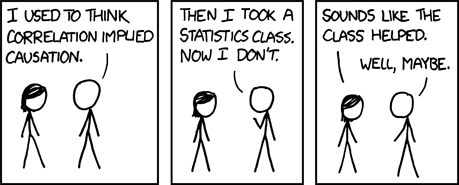
\includegraphics[width=12cm]{correlation.png}
\end{center}


\subsection{Exam, 27.12.2014 - solution}



\begin{enumerate}
\item $W_{\tau}$ takes values $100$ and $-100$ with equal probabilities. Yes, independent. $\E\left(  e^{-2\tau} \right) = \frac{2}{e^{200}+e^{-200}}$
\item $\E(S|N)=0.25N+0.5$, $\Var(S|N)=0.25N/12$, $\E(N)=1/p=2$, $\E(S)=\E(\E(S|N))=1$. One may also find the variance, $\Var(S)=1/8+1/24=1/6$.
\item By hints:
\begin{enumerate}
\item $d(tW_t)=t \, dW_t+W_t \, dt$
\item $\E\left(2t W_t\int_0^t s \, dW_s\right)=t^3$ using Ito's isometry
\item $\E\left(\left(\int_0^t s \, dW_s\right)^2 \right)=t^3/3$ using Ito's isometry
\item $\E\left(  \int_0^t W_s \, ds  \right)=0$
\item $\Var\left(  \int_0^t W_s \, ds  \right)=t^3/3$
\end{enumerate}
\item Event $\left\{ \frac{S_1-S_0}{S_0} < \frac{S_2-S_1}{S_1} \right\}$ simplifies to $S_1^2<S_0 S_2$ and further simplifies to $2\tilde{W}_1 - \tilde{W}_2 < 0$.

And
\[
X_0=e^{-0.2}\tilde{P}(2\tilde{W}_1 - \tilde{W}_2 < 0) = e^{-0.2}/2
\]

\item By steps:

\begin{enumerate}
\item Using the substitution $U_t=\ln Y_t$, one obtains the solution $Y_t=\exp(-W_t-t/2)$
\item $dA_t= Y_t (t-X_t)dt$
\item $f(t)=e^t$ for example
\item
\[
X_t=\frac{1+\int_0^t s \exp(-W_s+s/2) \, ds}{ \exp(-W_t +t/2 )}
\]
\end{enumerate}


\end{enumerate}



\end{document}
